\documentclass[11pt]{article}

\usepackage[margin=1in]{geometry}
\usepackage{amsmath,amssymb,amsfonts,bm,booktabs,array,enumitem,graphicx,hyperref,makeidx}
\usepackage[T1]{fontenc}
\usepackage{lmodern}
\usepackage{microtype}
\setlist[itemize]{leftmargin=2em}
\setlist[enumerate]{leftmargin=2em}
\setlength{\parskip}{0.45em}
\setlength{\parindent}{0pt}
\makeindex

\newcommand{\Unif}{\operatorname{Unif}}
\newcommand{\bSigma}{\bm{\Sigma}}
\newcommand{\ba}{\bm{a}}
\newcommand{\bb}{\bm{b}}
\newcommand{\balpha}{\bm{\alpha}}
\newcommand{\bbeta}{\bm{\beta}}
\newcommand{\bgamma}{\bm{\gamma}}
\newcommand{\bGamma}{\bm{\Gamma}}
\newcommand{\bdelta}{\bm{\delta}}
\newcommand{\beps}{\bm{\varepsilon}}
\newcommand{\btheta}{\bm{\theta}}
\newcommand{\bLambda}{\bm{\Lambda}}
\newcommand{\blambda}{\bm{\lambda}}
\newcommand{\bmu}{\bm{\mu}}
\newcommand{\bomega}{\bm{\omega}}
\newcommand{\bpi}{\bm{\pi}}
\newcommand{\bpsi}{\bm{\psi}}
\newcommand{\bp}{\bm{p}}
\newcommand{\bq}{\bm{q}}
\newcommand{\br}{\bm{r}}
\newcommand{\bu}{\bm{u}}
\newcommand{\bv}{\bm{v}}
\newcommand{\bw}{\bm{w}}
\newcommand{\bx}{\bm{x}}
\newcommand{\by}{\bm{y}}
\newcommand{\bz}{\bm{z}}
\newcommand{\bA}{\bm{A}}
\newcommand{\bB}{\bm{B}}
\newcommand{\bD}{\bm{D}}
\newcommand{\bF}{\bm{F}}
\newcommand{\bG}{\bm{G}}
\newcommand{\bI}{\bm{I}}
\newcommand{\bL}{\bm{L}}
\newcommand{\bQ}{\bm{Q}}
\newcommand{\bR}{\bm{R}}
\newcommand{\bV}{\bm{V}}
\newcommand{\bX}{\bm{X}}
\newcommand{\bZ}{\bm{Z}}
\newcommand{\bzero}{\bm{0}}
\newcommand{\bs}{\bm{s}}
\newcommand{\bo}{\bm{o}}
\newcommand{\bP}{\bm{P}}
\newcommand{\bH}{\bm{H}}
\newcommand{\bOmega}{\bm{\Omega}}
\newcommand{\bkappa}{\bm{\kappa}}
\newcounter{sampleralgorithm}
\newenvironment{sampleralgorithm}[2]{%
  \par\medskip\noindent\begin{minipage}{\linewidth}
  \refstepcounter{sampleralgorithm}\hrule\smallskip
  \noindent\textbf{Algorithm \thesampleralgorithm: #1}\par\smallskip\hrule\medskip
  #2\par
  \end{minipage}\par\medskip
}{\par\smallskip\hrule\medskip}
\newcommand{\trans}{^\top}
\newcommand{\Normal}{\operatorname{N}}
\newcommand{\Poisson}{\operatorname{Poisson}}
\newcommand{\NB}{\operatorname{NB}}
\newcommand{\Mult}{\operatorname{Multinomial}}
\newcommand{\Bin}{\operatorname{Binomial}}
\newcommand{\logit}{\operatorname{logit}}
\newcommand{\PG}{\operatorname{PG}}
\newcommand{\NNGP}{\operatorname{NNGP}}

\hypersetup{
  colorlinks=true,
  linkcolor=blue,
  citecolor=blue,
  urlcolor=blue
}

\title{\texttt{magComp}: Methods and Implementation Details}
\author{Andrew O. Finley}
\date{Updated \today}

% Cover-page logo width.
\newcommand{\coverlogowidth}{0.38\textwidth}

\begin{document}
\pagenumbering{gobble}
\begin{titlepage}
  \centering
  \vspace*{1.0in}
  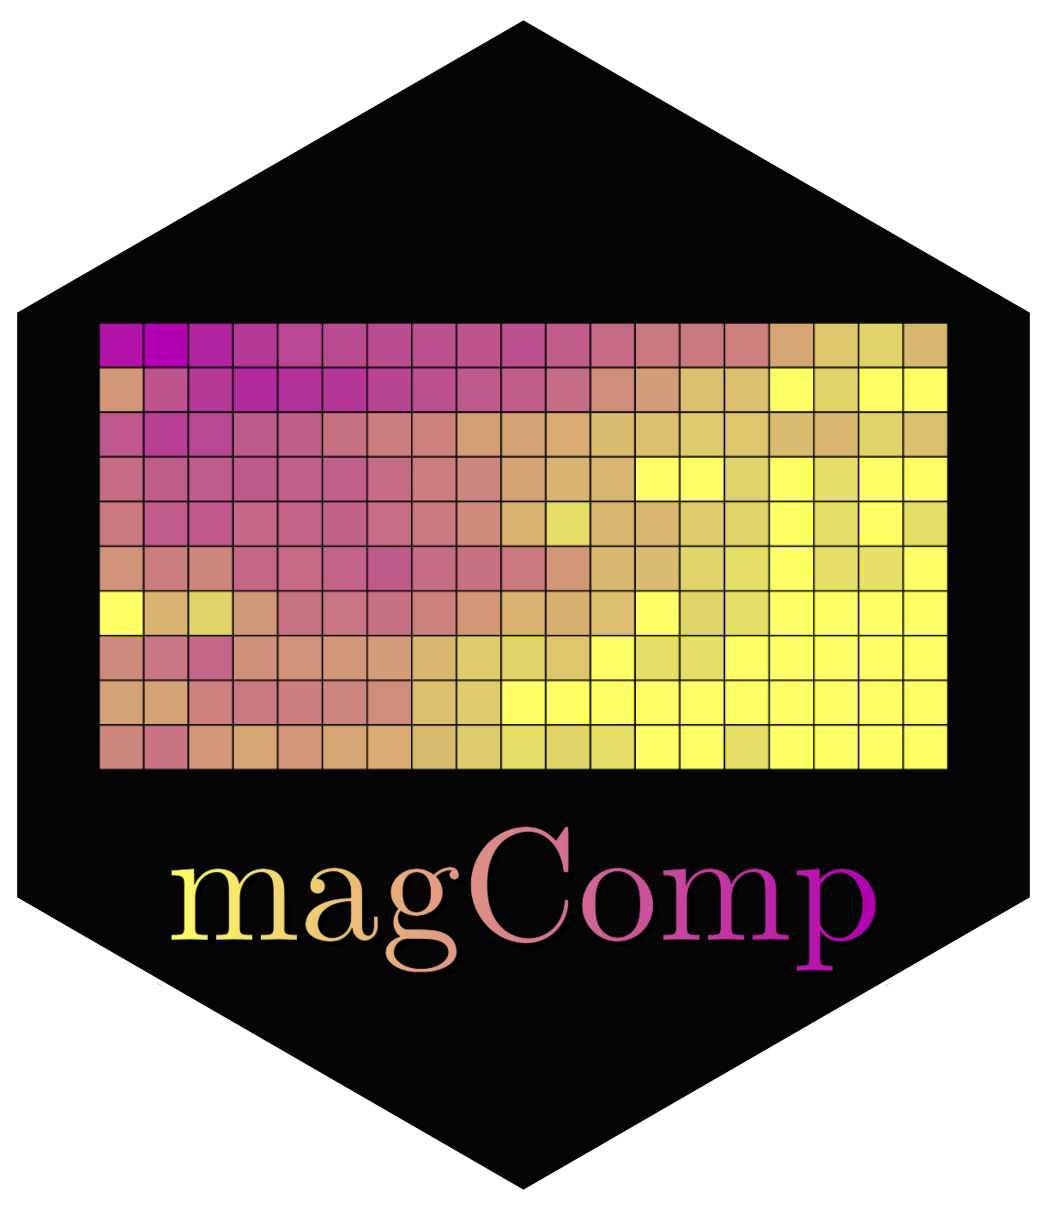
\includegraphics[width=\coverlogowidth]{logo.png}\par
  \vspace{0.35in}
  {\LARGE Methods and Implementation Details\par}
  \vspace{0.55in}
  {\large Andrew O. Finley\par}
  \vspace{0.25in}
  {\large Updated \today\par}
  \vfill
\end{titlepage}

\clearpage
\pagenumbering{roman}
\tableofcontents
\clearpage
\pagenumbering{arabic}

\section{Motivation and overview}
\index{overview}
\index{magnitude-composition model}

The \texttt{magComp} package fits Bayesian magnitude-composition models for
multivariate quantities observed over sampling units, spatial locations, or
prediction cells. The motivating application is forest inventory stand-table
prediction, where total abundance or another scalar forest attribute must be
allocated among diameter classes. The same model structure applies to other
settings where a nonnegative total and a category composition are jointly
modeled.

For sampling unit \(i=1,\ldots,n\) and category \(j=1,\ldots,J\), the mean
response is decomposed as
\begin{equation}
  \mu_{ij} = M_i p_{ij},
  \qquad
  p_{ij}\geq 0,
  \qquad
  \sum_{j=1}^{J}p_{ij}=1.
  \label{eq:magcomp-mean}
\end{equation}
The scalar \(M_i\) is the magnitude component. The implemented forest inventory
models use stem density for fixed-area plots and basal-area density for
horizontal point sampling. The vector \(\bp_i=(p_{i1},\ldots,p_{iJ})\trans\) is
the composition component, which allocates the magnitude among DBH classes or
other categories.

The decomposition in Equation~\ref{eq:magcomp-mean} separates two inferential
tasks. The magnitude model estimates the amount of material at a location or in
a sampling unit. The composition model estimates how that material is divided
among categories. This separation is useful when covariates explain total
amount differently than they explain category allocation, and when prediction
requires aggregation over many small spatial supports.

Users specify separate formulas for the magnitude and composition components. Each component can include fixed effects, unstructured
random effects, spatial effects, and varying-coefficient terms appropriate to
that component. Setting \texttt{composition = NULL} fits magnitude alone;
setting \texttt{magnitude = NULL} fits composition alone. An omitted formula
still defaults to an intercept, so disabling a component requires explicit
\texttt{NULL}. At least one component must be fitted.

\section{Data structure and notation}
\index{data structure}
\index{tree list}

The primary data structure is a tree list or event list with a sampling-unit
identifier. Let \(\bs_i\) denote the spatial location or centroid for sampling
unit \(i\), and let \(g(i)\) denote an optional group, stand, or stratum label.
Tree-level records supply category membership, such as species or DBH class,
and the unit's sampling information and covariates.
Aggregated integer counts can be supplied through \texttt{tree\_count}.
A magnitude-only analysis may omit categories and supply total counts per
unit; when categories are present, their counts are summed. A composition-only
analysis requires category counts but needs no area or BAF for fitting.
An empty sampling unit must still have a record with \texttt{tree\_count = 0}
and valid category and unit metadata; a unit absent from the input has no
likelihood contribution.

For fixed-area stem counts, \(y_{ij}\) is the integer number of trees observed
in unit \(i\) and category \(j\). The observed total is
\begin{equation}
  N_i = \sum_{j=1}^{J}y_{ij}.
  \label{eq:observed-total}
\end{equation}
The model notation uses \(\bz_i\) for magnitude predictors and \(\bx_i\) for
composition predictors. The two predictor sets may be identical, overlap, or be
disjoint. This distinction keeps the scientific interpretation explicit: a
covariate can influence the total amount, the allocation among categories, or
both.

Magnitude regression coefficients are \(\bbeta\); composition intercepts and slopes are
\(\alpha_{0j}\) and \(\balpha_j\). Magnitude iid and spatial effects are
\(\delta_g\) and \(v(\bs)\). Composition iid factors \(\bu_h\) have loadings
\(\bgamma_j\), whereas spatial factors \(\bw(\bs)\) have loadings
\(\blambda_j\). The grouping maps \(g(i)\) and \(h(i)\) may differ.
Additional terms and allocation blocks receive corresponding term and block
indices. Section~\ref{sec:software-notation} connects these symbols to the
software names.

\section{Fixed-area count model}
\index{fixed-area plots}
\index{stem counts}
\index{Poisson model}
\index{negative-binomial model}

For a fixed-area sampling unit with common tree-observation area \(a_i\) across
all categories, the total observed count is modeled with a negative-binomial
magnitude likelihood,
\begin{equation}
  N_i \mid M_i,r_M \sim \NB(a_i M_i,r_M),
  \label{eq:fixed-area-total}
\end{equation}
where \(M_i\) is stem density per unit area and \(r_M>0\) is the
negative-binomial size parameter. The package uses the mean-size
parameterization,
\begin{equation}
  E(N_i\mid M_i,r_M)=a_iM_i,
  \qquad
  \operatorname{Var}(N_i\mid M_i,r_M)
    =
    a_iM_i + \frac{(a_iM_i)^2}{r_M}.
  \label{eq:nb-mean-size}
\end{equation}
The Poisson model is the limiting case as \(r_M\rightarrow\infty\).
The package uses a finite size for fitting and prediction; its prior and
fixed-size option are described in Section~\ref{sec:size-priors}.

The log-density linear predictor is
\begin{equation}
  \log M_i
    =
    \bz_i\trans\bbeta
    + \delta_{g(i)}
    + v(\bs_i)
    + \sum_{q=1}^{p_M} z_{iq} v_{q}(\bs_i).
  \label{eq:magnitude-linear}
\end{equation}
The term \(\bz_i\trans\bbeta\) contains fixed effects, including an
intercept. The optional term \(\delta_{g(i)}\) is an iid group-level random
effect. The optional term \(v(\bs_i)\) is a spatial random intercept. The
optional terms \(v_{q}(\bs_i)\) are spatially varying coefficients.

Conditional on \(N_i\), the observed class-count vector follows a multinomial
allocation model,
\begin{equation}
  (y_{i1},\ldots,y_{iJ})\mid N_i,\bp_i
  \sim
  \Mult(N_i,\bp_i).
  \label{eq:composition-multinomial}
\end{equation}
The multinomial is represented through sequential binomials. Define the number
remaining before category \(j\) as
\begin{equation}
  R_{ij}=N_i-\sum_{h<j}y_{ih},
  \qquad
  j=1,\ldots,J-1.
  \label{eq:remaining-count}
\end{equation}
Then
\begin{equation}
  y_{ij}\mid R_{ij},\pi_{ij}
  \sim
  \Bin(R_{ij},\pi_{ij}),
  \qquad
  j=1,\ldots,J-1,
  \label{eq:sequential-binomial}
\end{equation}
and the final class receives the remaining count, \(y_{iJ}=R_{i,J-1}-y_{i,J-1}\). The continuation-ratio
probabilities \(\pi_{ij}\) are transformed to category probabilities by
\begin{equation}
  p_{ij} =
  \pi_{ij}\prod_{h<j}(1-\pi_{ih}),
  \qquad
  j=1,\ldots,J-1,
  \label{eq:stick-p}
\end{equation}
with
\begin{equation}
  p_{iJ} =
  \prod_{h<J}(1-\pi_{ih}).
  \label{eq:stick-final}
\end{equation}
Equations~\ref{eq:stick-p} and \ref{eq:stick-final} imply
\(\sum_{j=1}^{J}p_{ij}=1\) by construction.

The composition linear predictor is
\begin{equation}
  \psi_{ij}
  =
  g_C(\pi_{ij})
  =
  \alpha_{0j}
  + \bx_i\trans\balpha_j
  + \bgamma_j\trans\bu_{h(i)}
  + \sum_{q=1}^{p_C}
      x_{iq}\bgamma_{jq}\trans
      \bu_{q,h(i)}
  + \blambda_j\trans\bw(\bs_i)
  + \sum_{q=1}^{p_C}
      x_{iq}\blambda_{jq}\trans
      \bw_{q}(\bs_i).
  \label{eq:composition-linear}
\end{equation}
where \(g_C\) is either the logit link or the probit link selected by
\texttt{control\$composition\_link}. The inverse link is therefore
\(g_C^{-1}(\psi)=\Phi(\psi)\) for the default probit model and
\(g_C^{-1}(\psi)=\{1+\exp(-\psi)\}^{-1}\) for the optional logit model.
The coefficients \(\alpha_{0j}\) are category-specific intercepts.
The vector \(\balpha_j\) contains category-specific fixed slopes. The optional
term \(\bgamma_j\trans\bu_{h(i)}\) is an unstructured factor random effect.
The first summation provides group-varying composition coefficients through
unstructured factor scores.
The optional term \(\blambda_j\trans\bw(\bs_i)\) is a spatial factor
effect. The final summation provides spatially varying composition
coefficients through factor processes.

\subsection{Two-category conditional composition}
\index{conditional composition}
\index{two-category tables}
\index{allocation blocks}

The same magnitude-composition decomposition applies when each response cell is
defined by two categorical variables. Let \(A\) have levels
\(a=1,\ldots,J_A\), and let \(B\) have levels \(b=1,\ldots,J_B\). The cell mean
is
\begin{equation}
  \mu_{iab}=M_i p_{iab},
  \qquad
  a=1,\ldots,J_A,
  \qquad
  b=1,\ldots,J_B.
  \label{eq:two-category-mean}
\end{equation}
This covers species-group-by-DBH stand tables, but the notation is generic:
\(A\) and \(B\) can be any two categorical response dimensions.

The implemented two-category model uses a conditional factorization,
\begin{equation}
  p_{iab}=q_{ia}r_{ib\mid a},
  \label{eq:conditional-factorization}
\end{equation}
where
\begin{equation}
  q_{ia}=P(A_i=a),
  \qquad
  r_{ib\mid a}=P(B_i=b\mid A_i=a).
  \label{eq:conditional-components}
\end{equation}
Users choose which variable is \(A\) by listing it first in
\texttt{categories}; the second variable is modeled conditionally on the first.
Either variable can be ordered or unordered. Reversing the category columns
and the corresponding composition formulas fits the reverse conditioning,
\(B\) then \(A\mid B\). These are different model specifications and need not
give equivalent fits under structured predictors or priors. For forest stand
tables, a natural choice is a nominal leading category, such as species group,
followed by an ordered child category, such as DBH class.
For nominal leading categories, the continuation-ratio representation is
conditional on the user-specified level order. This ordering does not affect the
ability of a saturated model to represent a multinomial distribution, but fitted
covariate effects and random-effect loadings can depend on the chosen order when
structure or shrinkage is imposed. Sensitivity to nominal category ordering is
therefore a useful diagnostic when the leading margin is unordered.

Define the probability vectors
\(\bq_i=(q_{i1},\ldots,q_{iJ_A})\trans\) and
\(\br_{i\cdot\mid a}=(r_{i1\mid a},\ldots,r_{iJ_B\mid a})\trans\).
Let \(y_{ia+}=\sum_{b=1}^{J_B}y_{iab}\),
\(\by_{iA+}=(y_{i1+},\ldots,y_{iJ_A+})\trans\), and
\(\by_{iaB}=(y_{ia1},\ldots,y_{iaJ_B})\trans\).
The likelihood is represented by two allocation blocks. The first allocates
the total count among the categories of \(A\),
\begin{equation}
  \by_{iA+}\mid N_i,\bq_i
  \sim
  \Mult(N_i,\bq_i),
  \label{eq:leading-margin}
\end{equation}
and the second allocates each parent count among the categories of \(B\),
\begin{equation}
  \by_{iaB}\mid y_{ia+},\br_{i\cdot\mid a}
  \sim
  \Mult(y_{ia+},\br_{i\cdot\mid a}),
  \qquad
  a=1,\ldots,J_A.
  \label{eq:child-conditional}
\end{equation}
If \(y_{ia+}=0\), the corresponding child allocation contributes no likelihood
information for unit \(i\) and leading level \(a\).

Each allocation block is fit using the sequential-binomial representation in
Equations~\ref{eq:remaining-count}--\ref{eq:stick-final}. Thus the leading
allocation has \(J_A-1\) continuation-ratio linear predictors, and the child
allocation has \(J_A(J_B-1)\) linear predictors when child-category parameters
are allowed to vary by leading level. Fixed effects, smoothing, iid factor
terms, GP factor terms, and NNGP factor terms are attached to allocation
blocks.

The predictor vectors \(\bx_i^{(A)}\) and \(\bx_i^{(B\mid A)}\) can differ.
Each parent has its own child coefficients and loading rows, while each child
factor term shares its score vectors across parents. Thus species-specific
size distributions can load
differently on common group-level or spatial patterns.

Equations~\ref{eq:fixed-area-total}, \ref{eq:leading-margin}, and
\ref{eq:child-conditional} imply the parent-level and cell-level means
\begin{equation}
  E(y_{ia+}\mid M_i,\bq_i)=a_iM_iq_{ia}
  \label{eq:implied-parent-mean}
\end{equation}
and
\begin{equation}
  E(y_{iab}\mid M_i,\bq_i,\br_{i\cdot\mid a})=a_iM_iq_{ia}r_{ib\mid a}.
  \label{eq:implied-cell-mean}
\end{equation}
The total count is modeled once, then allocated through the composition blocks.

\subsection{Fixed-area support and nested plots}
\index{nested fixed-area plots}
\index{fixed-area support}

The count likelihood requires a common observation area \(a_i\) across
categories within a sampling unit. It does not accept a unit-by-category
matrix of areas. For nested regeneration, sapling, and overstory subplots,
stem-count analyses must first define a common support. Tree expansion
factors do not make counts from unequal category-specific areas compatible
with this likelihood.

\section{Point-sampling basal area}
\label{sec:point-sampling}
\index{horizontal point sampling}
\index{tree factor}

The point-sampling family models basal-area density using horizontal
point-sampling tally counts.

For horizontal point sampling with basal area factor
\(\operatorname{BAF}_i\), a tree with basal area \(\mathrm{BA}_{it}\) has tree factor
\begin{equation}
  \mathrm{TF}_{it} = \frac{\operatorname{BAF}_i}{\mathrm{BA}_{it}}.
  \label{eq:point-tree-factor}
\end{equation}
This expansion factor converts an observed in-tree to a per-unit-area tree
count contribution. Other attributes expanded with these tree factors are outside the
implemented count likelihood; see Section~\ref{sec:implementation-limits}.

Basal area under horizontal point sampling is a special count-based case. The
number of in-trees at point \(i\), denoted \(m_i\), satisfies
\begin{equation}
  m_i\mid M_i^{BA},r_M^{BA}
  \sim
  \NB\left(\frac{M_i^{BA}}{\operatorname{BAF}_i},r_M^{BA}\right),
  \label{eq:point-ba-count}
\end{equation}
where \(M_i^{BA}\) is basal area per unit area. The magnitude component in
Equation~\ref{eq:magnitude-linear} can be used for \(\log M_i^{BA}\), and the
composition component allocates basal area among categories. The
negative-binomial variance is
\(M_i^{BA}/\operatorname{BAF}_i + (M_i^{BA}/\operatorname{BAF}_i)^2/r_M^{BA}\), with the
Poisson point-sampling tally model recovered as \(r_M^{BA}\rightarrow\infty\).

This point-sampling model does not explicitly account for forest boundaries
that truncate tree inclusion zones. Restricting tallies to forest trees near a
boundary can reduce expected counts even when basal-area density is unchanged.
The reduction depends on tree size and is not generally captured by a single
area adjustment. Stand or forest inference from such points requires additional
modeling of these boundary effects.

\section{Model terms}
\label{sec:model-terms}
\index{model terms}
\index{formula interface}
\index{factor model}

Fixed effects use ordinary R formula syntax. Magnitude effects enter the
log-density predictor; composition effects enter each allocation block's
continuation-ratio predictors. The following terms specify random intercepts
or factor contributions, with \texttt{s1} and \texttt{s2} denoting coordinate
columns. Additional coordinate columns are allowed.

\begin{center}
\small
\begin{tabular}{@{}lp{0.48\linewidth}p{0.31\linewidth}@{}}
\toprule
Component & Formula term & Contribution \\
\midrule
Magnitude & \texttt{iid(group)} & Iid group effect \\
 & \texttt{gp(s1, s2)} & Dense GP effect \\
 & \texttt{nngp(s1, s2, m = 15)} & NNGP effect \\
Composition & \texttt{factor\_iid(group, K = 2)} & \(K\) iid group factors \\
 & \texttt{factor\_gp(s1, s2, K = 2)} & \(K\) dense GP factors \\
 & \texttt{factor\_nngp(s1, s2, K = 2, m = 15)} & \(K\) NNGP factors \\
\bottomrule
\end{tabular}
\end{center}

Prefixing any term with \texttt{x:} multiplies its contribution by covariate
\texttt{x}, giving a group-varying or spatially varying coefficient. Include
\texttt{x} separately in the fixed-effect formula when an average fixed slope
is desired. For example, \texttt{x:iid(group)} gives an iid magnitude slope,
and \texttt{x:factor\_nngp(s1, s2, K = 2)} gives a spatial composition slope.

Multiple process terms may enter additively. For composition block \(C\),
let \(\mathcal T_C^u\) and \(\mathcal T_C^w\) denote its iid and spatial
terms. Their combined contribution is
\begin{equation}
 f_{ij}^{(C)}=
 \sum_{t\in\mathcal T_C^u}d_{it}^{(C)}\bgamma_{jt}\trans\bu_{t,h_t(i)}
 +\sum_{t\in\mathcal T_C^w}d_{it}^{(C)}\blambda_{jt}\trans\bw_t(\bs_i).
 \label{eq:additive-composition-factor-terms}
\end{equation}
Here \(d_{it}^{(C)}=1\) for an intercept term and equals the covariate for
a varying-coefficient term. Each term has its own rank, loading matrix, scores,
anchors, and covariance parameters when applicable. Increasing rank permits richer
residual dependence across categories. Section~\ref{sec:factor-identification}
defines the loading constraints. In conditional blocks, parent-specific
loading rows act on shared scores as described in the two-category model.

\section{Factor identification}
\label{sec:factor-identification}
\index{factor identification}
\index{loading matrix}

For a \(K\)-factor spatial composition term, collect the loadings in the
\(L\times K\) matrix
\begin{equation}
  \bLambda =
  \begin{bmatrix}
    \blambda_1\trans\\
    \vdots\\
    \blambda_L\trans
  \end{bmatrix}.
  \label{eq:loading-matrix}
\end{equation}
For a one-category allocation block, \(L=J-1\). For a conditional
\(B\mid A\) block with parent-specific child stick rows, \(L=J_A(J_B-1)\), with
rows ordered by the parent-child stick labels described in
Equation~\ref{eq:child-conditional}.
Independent spatial factors have unit-scale parent GP correlation functions,
with NNGP approximations where specified. Iid factors are independent standard
normals; their loading matrix \(\bGamma\) uses the same constraints, with
\(\gamma\) replacing \(\lambda\) below.
The implementation selects \(K\) ordered anchor rows. If
\(a_1,\ldots,a_K\) are the anchor row indices, then
\begin{equation}
  \lambda_{a_k,h}=0 \quad(h>k),\qquad \lambda_{a_k,k}>0.
  \label{eq:triangular-zero}
\end{equation}
After placing the anchor rows first in their specified order, their submatrix
is lower triangular with positive diagonal.
Non-anchor rows have unrestricted loadings.
Anchor rows, their order, and factor rank are reported as part of the model
specification. For an iid intercept factor term this gives within-group
covariance \(\bGamma\bGamma\trans\); for a dense-GP intercept factor term,
the within-location covariance is \(\bLambda\bLambda\trans\). The first anchor's
factor contribution has variance equal to its squared diagonal loading.
The NNGP version uses the corresponding unit-scale parent-GP approximation.
The factor scale is fixed while the loadings determine the amplitude.
The positive-diagonal constraints follow the residual-factor construction
in Taylor-Rodriguez et al. (2019, Appendix B).

When anchors are omitted, the software ranks stick rows by the trial-weighted
variance of empirical logits \(\logit\{(y+0.5)/(R+1)\}\), even for a probit
fit, and fills any remaining slots in row order. Conditional blocks rank all
parent-child stick rows.

\section{Prior distributions}
\label{sec:priors}
\index{prior distributions}

\subsection{Regression coefficients and ordered-category smoothing}
\label{sec:smoothing}
\index{smoothing}
\index{random walk priors}
\index{DBH classes}

Fixed-effect coefficients in the magnitude component have normal priors,
\begin{equation}
  \bbeta \sim \Normal(\bzero,\sigma_\beta^2\bI).
  \label{eq:magnitude-coefficient-prior}
\end{equation}
Here \(\sigma_\beta^2\) is
\texttt{magnitude\$coefficient\_variance} in the prior list.
The interface does not accept arbitrary prior means or covariance matrices.
Without smoothing, composition intercepts and slopes have independent
normal priors,
\begin{equation}
  \alpha_{0j}\sim\Normal(0,\sigma_{\alpha,0}^2),
  \qquad
  \balpha_j\sim\Normal(\bzero,\sigma_\alpha^2\bI).
  \label{eq:composition-coefficient-prior}
\end{equation}
The software settings \texttt{intercept\_variance} and
\texttt{slope\_variance} specify \(\sigma_{\alpha,0}^2\) and
\(\sigma_\alpha^2\), respectively. For an ordered block, let
\(\btheta_q=(\theta_{q1},\ldots,\theta_{q,J-1})\trans\) collect its
intercepts (\(q=0\), \(\theta_{0j}=\alpha_{0j}\)) or one predictor's
slopes (\(q>0\), \(\theta_{qj}\) is element \(q\) of \(\balpha_j\)).
For indices within the coefficient vector, the difference matrices act as
\[
 (\bD_1\btheta_q)_j=\theta_{q,j+1}-\theta_{qj},\qquad
 (\bD_2\btheta_q)_j=\theta_{q,j+2}-2\theta_{q,j+1}+\theta_{qj}.
\]
RW1 penalizes adjacent differences; RW2 penalizes changes in adjacent slopes.
The complete proper prior is
\begin{equation}
 \btheta_q\sim\Normal(\bzero,\bP_q^{-1}),\qquad
 \bP_q=\bV_q^{-1}+\tau_q^{-2}\bD_{d_q}\trans\bD_{d_q},
 \label{eq:proper-smoothing-prior}
\end{equation}
where \(d_q\) is the selected difference order,
\(\bV_0=\sigma_{\alpha,0}^2\bI\), and
\(\bV_q=\sigma_\alpha^2\bI\) for slopes. Omit the difference term when
smoothing is disabled. The normal base precision makes the prior proper;
the difference penalty alone would be singular. Smoothing variances are fixed
hyperparameters: \texttt{intercept\_smoothing\_variance} specifies
\(\tau_0^2\), and \texttt{slope\_smoothing\_variance} supplies a common
value for the slope vectors within a block.

Child coefficient vectors are smoothed separately within each parent, so their
joint prior precision is block diagonal over parents. No difference penalty
crosses a parent boundary. Smoothing acts on continuation-ratio coefficients;
the nonlinear transforms in Equations~\ref{eq:stick-p} and
\ref{eq:stick-final} need not produce smooth category proportions.

\subsection{Factor loadings}

Estimated off-diagonal iid and spatial loading elements have
priors \(\gamma_{jk}\sim\Normal(0,c_\gamma)\) and
\(\lambda_{jk}\sim\Normal(0,c_\lambda)\), respectively. Each term's
\texttt{loading\_variance} specifies its corresponding \(c_\gamma\) or
\(c_\lambda\), with block defaults and per-term overrides. Each anchor-diagonal
loading has the corresponding normal prior restricted to \((0,\infty)\).
The setting is the normal variance before truncation, so a value \(c\)
gives half-normal scale \(\sqrt c\). The default is one.

\subsection{Size and latent process priors}
\label{sec:size-priors}

When the magnitude negative-binomial size is estimated, it has a Gamma prior,
\begin{equation}
  r_M \sim \operatorname{Gamma}(a_r,b_r),
  \label{eq:nb-size-prior}
\end{equation}
using the shape-rate convention. The automatic setting
\texttt{priors\$magnitude\$size = "auto"} estimates size with
\((a_r,b_r)=(1,0.01)\) when the magnitude formula has no iid or spatial
terms, and otherwise fixes size at \texttt{control\$nb\_size} (default 1000).
This policy applies to fixed-area and point-sampling models. Composition
factor terms do not restrict size estimation.
Its shape and rate can be changed through \texttt{magCompPriors()}.
An explicit \texttt{size = NULL} fixes size. Joint estimation of size and
magnitude random-effect terms is not supported.

For magnitude iid term \(t\), including an intercept or varying slope,
\begin{equation}
  \delta_{gt} \mid \sigma_{\delta,t}^2 \sim \Normal(0,\sigma_{\delta,t}^2),
  \qquad
  \sigma_{\delta,t}^2 \sim \operatorname{IG}(a_\delta,b_\delta).
  \label{eq:iid-prior}
\end{equation}
Each term has a separate variance, with default inverse-gamma shape and scale
\((a_\delta,b_\delta)\) supplied by \texttt{magnitude\$iid\_variance}, defaulting to \((2,1)\). A named magnitude term can override these hyperparameters.
For a spatial magnitude random effect,
\begin{equation}
  \bv \mid \sigma_v^2,\phi_v
  \sim
  \Normal\{\bzero,\sigma_v^2\bR(\phi_v)\},
  \label{eq:spatial-prior}
\end{equation}
where \(\bv=(v(\bs_1),\ldots,v(\bs_n))\trans\) and \(\bR(\phi_v)\) is a
spatial correlation matrix or its NNGP approximation.
For each magnitude GP or NNGP term, including a varying slope, the variance prior is
\begin{equation}
  \sigma_v^2 \sim \operatorname{IG}(a_\sigma,b_\sigma),
  \label{eq:magnitude-nngp-variance-prior}
\end{equation}
which gives a Gibbs update conditional on \(\bv\) and \(\phi_v\).
Here \(\operatorname{IG}(a,b)\) has density proportional to
\(x^{-a-1}\exp(-b/x)\), and its shape and scale are supplied by
\texttt{magnitude\$spatial\_variance}, with named per-term overrides.
For a composition spatial factor term, the sampler uses independent
unit-variance parent GP priors for the factor columns,
\begin{equation}
  \bw_k
  \mid \phi_{w,k}
  \sim
  \Normal\{\bzero,\bR(\phi_{w,k})\},
  \qquad
  k=1,\ldots,K.
  \label{eq:composition-factor-nngp-prior}
\end{equation}
Here \(\bw_k=(w_k(\bs_1),\ldots,w_k(\bs_n))\trans\) contains factor \(k\)
over the observed locations. For \texttt{factor\_nngp()}, this full spatial prior is replaced by the NNGP
conditional approximation.

\subsection{Spatial and space-time covariance families}
\label{sec:covariance-families}

The exponential correlation is the default. The same covariance registry
supports dense GP and NNGP terms in magnitude, leading allocation, and
conditional allocation models, including varying coefficients. Write
\(h=\|\bs-\bs'\|\), \(u=|t-t'|\), and let \(d_s\) be the number of spatial
coordinates. The available unit-variance correlations are
\begin{align}
 \rho_{\mathrm{exp}}(h;\phi)&=\exp(-\phi h),\\
 \rho_{\mathrm{Mat}}(h;\phi,\nu)&=
   \frac{(\phi h)^\nu K_\nu(\phi h)}{2^{\nu-1}\Gamma(\nu)},\\
 \rho_{\mathrm{sep}}(h,u;\phi,\lambda)&=\exp(-\phi h-\lambda u),\\
 \rho_{\mathrm{mix}}(h,u)&=\alpha\exp(-\phi_1h-\lambda_1u)
                   +(1-\alpha)\exp(-\phi_2h-\lambda_2u),\\
 \rho_{\mathrm{G}}(h,u)&=T^{-\delta-d_s/2}
                  \exp\{-c h^{2\gamma}/T^{\beta\gamma}\},
       \qquad T=1+a u^{2\alpha}.
 \label{eq:covariance-registry}
\end{align}
The Mat\'ern correlation is one at zero distance and reduces to the exponential
at \(\nu=1/2\). For the Gneiting (2002) family, \(a,c>0\),
\(0<\alpha,\gamma\leq1\), \(0\leq\beta\leq1\), and \(\delta\geq0\).
All decay parameters and Mat\'ern smoothness are positive; the mixture weight
lies in \([0,1]\). Magnitude variance remains a separate parameter, while
composition factor correlations have unit marginal variance.

Use \texttt{cov\_model = "exp"}, \texttt{"matern"}, \texttt{"sep\_exp"},
\texttt{"multi\_res\_sep\_exp"}, or \texttt{"gneiting"} in a process term.
For a space-time family the final coordinate is numeric time, for example
\texttt{nngp(easting, northing, year, cov\_model = "sep\_exp")}.
Actual time gaps enter the covariance. NNGP neighbor search uses
\(\{h^2+(s_{\mathrm{search}}u)^2\}^{1/2}\), where the positive
\texttt{st\_scale} setting defaults to one. This setting affects the directed
neighbor graph only; correlations always use the original spatial and temporal
lags. The graph is fixed during sampling, and prediction inherits its search
scale. Different sampling units must have distinct full coordinate tuples;
space-time models therefore permit revisits at different dates, but a
spatial-only term cannot represent those revisits as separate latent nodes.

\subsection{Covariance priors and settings}

Each magnitude process term and each composition factor has its own covariance
parameter vector, denoted \(\boldsymbol\vartheta\) below. Every estimated
entry has an independent bounded uniform prior. Priors, starts, and initial
proposal standard deviations share a term's named \texttt{covariance} list.
For example, \texttt{phi = uniform(0.1, 5)} specifies prior bounds,
\texttt{phi = 1} a starting value, and \texttt{phi = fixed(1)} a fixed value
in the starting list. Factor-specific named overrides are supported.
\texttt{magCompCovModels()} lists parameter names and domains;
\texttt{magCompSettings()} supplies resolved templates.

For automatic spatial bounds let \(D\) be maximum spatial separation and
\(r_0=\tfrac12\operatorname{median}_i d_i^{\mathrm{NN}}\), using distinct
spatial sites. For numerical scaling, replace \(r_0\) by at least
\(\sqrt{\epsilon_{\mathrm{machine}}}D\). Defaults for \texttt{exp},
\texttt{matern}, and \texttt{sep\_exp} are
\begin{equation}
 \phi\sim\Unif\{3/(2D),3/\min(r_0,D/2)\}.
 \label{eq:default-range-support}
\end{equation}
The initial value is \(6/D\), replaced by the support midpoint if needed.
For the mixture, \(\phi_1\sim\Unif(3/D,30/D)\) and
\(\phi_2\sim\Unif\{30/D,3/\min(r_0,0.05D)\}\), so component 1 describes
longer spatial dependence. The mixing weight has prior \(\Unif(0,1)\).
User-specified supports replace these defaults; overlapping component supports
can permit label switching.

If \(T_0\) is the time span and \(\Delta_0\) the smallest positive time gap,
temporal exponential decays have prior
\(\Unif\{3/(2T_0),6/\Delta_0\}\). This calibrates the upper extent of temporal
dependence to twice the observed time domain. Mat\'ern smoothness defaults to
\(\nu\sim\Unif(0.05,2)\). Gneiting defaults fix
\(\alpha=1,\gamma=1/2,\delta=0\), estimate \(\beta\sim\Unif(0,1)\), and use
the spatial \(\phi\) support for \(c\). Its default support for \(a\) is
\([C/(2T_0)^2,C/(\Delta_0/2)^2]\), with \(C=0.05^{-2/d_s}-1\), calibrated
at those default shape values. A prior or ordinary numeric start can release
a default-fixed shape parameter; \(\delta\) then defaults to \(\Unif(0,2)\).
Other automatic starts use support midpoints. If a coordinate domain has no
positive span, its corresponding support or fixed value must be supplied.
These are uniform priors on covariance parameters, not on effective ranges.

\section{Augmentation and sampler notation}
\label{sec:augmentation}
\index{Polya-Gamma}
\index{probit augmentation}
\index{MCMC}

The sampler retains magnitude random effects and composition factor scores as
latent variables. Conditional on augmentation variables, their likelihood
contributions are normal kernels. Section~\ref{sec:normal-draws} defines the
dense and sparse Cholesky draws used in the sampler.

\subsection{Magnitude augmentation}

Write \(e_i\) for the observation multiplier: \(e_i=a_i\) for fixed-area
plots and \(e_i=1/\operatorname{BAF}_i\) for point sampling. In the sampler
formulas, \(N_i\) denotes the observed total tally, \(M_i\) the corresponding
magnitude, and \(r_M\) the size. For point sampling these stand for
\(m_i\), \(M_i^{BA}\), and \(r_M^{BA}\), respectively.
The count mean is \(e_iM_i\). Define
\begin{equation}
  \eta_i^{(M)}=\log M_i,\qquad
  o_i^{(M)}=\log e_i-\log r_M,\qquad
  \psi_i^{(M)}=\eta_i^{(M)}+o_i^{(M)}.
  \label{eq:nb-logit}
\end{equation}
For fixed \(r_M\), the negative-binomial likelihood kernel is
\begin{equation}
  \frac{\exp\{N_i\psi_i^{(M)}\}}
       {\{1+\exp(\psi_i^{(M)})\}^{N_i+r_M}},
  \qquad \kappa_i^{(M)}=\frac{N_i-r_M}{2}.
  \label{eq:nb-pg-kappa}
\end{equation}
P\'olya--Gamma augmentation (Polson et al., 2013) gives
\begin{equation}
  \omega_i^{(M)}\mid\cdot\sim\PG(N_i+r_M,\psi_i^{(M)}),
  \qquad
  \mathcal K_i^{(M)}(\psi_i^{(M)})\propto\exp\!\left\{\kappa_i^{(M)}\psi_i^{(M)}
    -\frac{\omega_i^{(M)}}{2}(\psi_i^{(M)})^2\right\}.
  \label{eq:pg-magnitude}
\end{equation}
Here \(\mathcal K_i^{(M)}\) is the augmented joint-density kernel as a
function of the predictor, holding the count and augmentation draw fixed.

\subsection{Composition augmentation}

In each allocation block, use \(y_{ij}\), \(R_{ij}\), and \(\psi_{ij}\)
for the binomial count, remaining count, and continuation-ratio predictor.
Define weights \(\omega_{ij}\) and canonical linear terms \(h_{ij}\) so
that the augmented kernel is
\begin{equation}
  \exp\!\left\{h_{ij}\psi_{ij}-\frac{\omega_{ij}}2\psi_{ij}^2\right\}.
  \label{eq:composition-augmented-kernel}
\end{equation}
For the optional logit link,
\begin{equation}
  \omega_{ij}\mid\cdot\sim\PG(R_{ij},\psi_{ij}),\qquad
  h_{ij}=\kappa_{ij}^{(C)}=y_{ij}-R_{ij}/2.
  \label{eq:pg-composition}
\end{equation}

For the default probit link, introduce one latent normal for each of the
\(R_{ij}\) observations available at the allocation step.
Conditional on the count, draw \(y_{ij}\) independent
\(\Normal(\psi_{ij},1)\) variables restricted to \((0,\infty)\) and
\(R_{ij}-y_{ij}\) restricted to \((-\infty,0]\). This is the grouped-count
version of latent-normal probit augmentation (Albert and Chib, 1995;
Rouder and Lu, 2005). With latent values \(\zeta_{ijt}\), retain their sum,
\begin{equation}
  S_{ij}=\sum_{t=1}^{R_{ij}}\zeta_{ijt},\qquad
  h_{ij}=S_{ij},\qquad \omega_{ij}=R_{ij}.
  \label{eq:probit-latent-sum}
\end{equation}
The same normal coefficient, loading, and score updates then apply to both
links. When \(R_{ij}=0\), set
\(h_{ij}=\omega_{ij}=0\) and draw no augmentation variables.

\subsection{Indices, offsets, and spatial precision}
\label{sec:sampler-notation}

The following algorithm applies to every fitted allocation block. Within a
block, \(j\) indexes a coefficient/loading row. For a leading block these
are the \(J_A-1\) continuation-ratio rows; for a conditional block they are
the \(J_A(J_B-1)\) parent--child rows. Let \(\mathcal I_j\) contain the
data rows governed by coefficient row \(j\). A child data row represents a
sampling unit and parent context \((i,a)\); its group and spatial indices
refer back to the original sampling unit. Thus shared factor scores are
updated using contributions from all their associated parent contexts.

Write \(X_{iq}\) for the composition design entry, with \(X_{i0}=1\), and
\(\btheta_q\) for the coefficient vector over all \(L\) coefficient rows:
\(\theta_{0j}=\alpha_{0j}\), with \(q>0\) indexing slopes. The prior
precision \(\bP_q\) is defined in Equation~\ref{eq:proper-smoothing-prior};
for child blocks it contains one diagonal block per parent.
Let \(d_{it}\) denote a process term's covariate multiplier:
one for an intercept term and the specified covariate for a varying slope.
Offsets below always use the latest values of every component except the one
being updated.

For a spatial or space-time term with covariance parameters \(\boldsymbol\vartheta\), let \(\bH_{\boldsymbol\vartheta}\) denote its unit-scale prior precision,
and let \(d_{\boldsymbol\vartheta}\) denote the log determinant of its unit-scale covariance:
\begin{equation}
 \begin{aligned}
  \bH_{\boldsymbol\vartheta}&=\bR_{\boldsymbol\vartheta}^{-1}, &d_{\boldsymbol\vartheta}&=\log|\bR_{\boldsymbol\vartheta}| &&\text{(dense GP)},\\
  \bH_{\boldsymbol\vartheta}&=(\bI-\bB_{\boldsymbol\vartheta})\trans\bF_{\boldsymbol\vartheta}^{-1}(\bI-\bB_{\boldsymbol\vartheta}),
  &d_{\boldsymbol\vartheta}&=\sum_i\log F_i(\boldsymbol\vartheta) &&\text{(NNGP)}.
 \end{aligned}
 \label{eq:spatial-precision}
\end{equation}
NNGP locations are ordered by the first coordinate, with subsequent coordinates
breaking ties. Let \(\mathcal N_i\) be the at most \(m\) nearest earlier
locations under the search distance in Section~\ref{sec:covariance-families}. For the chosen unit-scale correlation, solve
\begin{equation}
  \bR_{\mathcal N_i,\mathcal N_i}\bb_i(\boldsymbol\vartheta)
                    =\bR_{\mathcal N_i,i},\qquad
  F_i(\boldsymbol\vartheta)=1-\bR_{i,\mathcal N_i}\bb_i(\boldsymbol\vartheta).
  \label{eq:nngp-conditional-parallel}
\end{equation}
Row \(i\) of \(\bB_{\boldsymbol\vartheta}\) contains \(\bb_i\trans\) in its neighbor
columns and zeros elsewhere; \(\bF_{\boldsymbol\vartheta}=\operatorname{diag}(F_i)\).
The first location has no neighbors and \(F_1=1\). In these equations vectors
are in spatial order. This conditional construction follows Finley et al. (2019).
For a spatial vector \(\bv\) with variance \(s^2\), its log prior, up to a
constant, is
\begin{equation}
  G(\bv;\boldsymbol\vartheta,s^2)
  =-\tfrac12\{n\log s^2+d_{\boldsymbol\vartheta}+s^{-2}\bv\trans\bH_{\boldsymbol\vartheta}\bv\}.
  \label{eq:spatial-log-prior}
\end{equation}
Use the vector's own number of locations for \(n\). Composition spatial
factors have \(s^2=1\).

\subsection{Normal draws using Cholesky solves}
\label{sec:normal-draws}
\index{CHOLMOD}

Each unrestricted normal update below specifies a precision \(\bQ\) and
linear term \(\bb\), defining the full conditional
\begin{equation}
 \boldsymbol\zeta\mid\cdot\sim\Normal(\bQ^{-1}\bb,\bQ^{-1}).
 \label{eq:gaussian-full-conditional}
\end{equation}
For Gibbs updates, \(\mid\cdot\) denotes conditioning on the data and latest
values of the other parameters and latent variables. The draw operations
below compute this distribution using solves, without forming its covariance.

For a dense precision, \(\mathcal G_D(\bQ,\bb)\) factors
\(\bQ=\bL\bL\trans\) and computes
\begin{equation}
 \begin{gathered}
  \bL\ba=\bb,\qquad \bL\trans\boldsymbol m=\ba,\qquad
  \bL\trans\boldsymbol e=\beps,\qquad \beps\sim\Normal(\bzero,\bI),\\
  \boldsymbol\zeta=\boldsymbol m+\boldsymbol e.
 \end{gathered}
 \label{eq:precision-draw}
\end{equation}
LAPACK performs the Cholesky factorization and mean solves; a BLAS triangular
solve supplies the random component. This operation is used for regression
coefficients, smoothed coefficient vectors, iid factor-score vectors, and
dense GP latent vectors. The coefficient draws use dense factorization even
when the smoothing prior precision is banded.

For an NNGP latent vector, the posterior precision has the sparse form
\begin{equation}
 \bQ_{\mathrm{post}}=s^{-2}\bH_{\boldsymbol\vartheta}+\operatorname{diag}(D_i),
 \label{eq:nngp-posterior-precision}
\end{equation}
where \(D_i\) collects the augmented-likelihood weights at location \(i\).
It is assembled directly from the neighbor conditionals and likelihood
contributions. For a sparse precision \(\bQ\),
\(\mathcal G_S(\bQ,\bb)\) uses CHOLMOD's fill-reducing permutation
\(\boldsymbol\Pi\) and factorization
\(\boldsymbol\Pi\bQ\boldsymbol\Pi\trans=\bL\bL\trans\) to compute
\begin{equation}
 \begin{gathered}
  \bL\ba=\boldsymbol\Pi\bb,\qquad
  \bL\trans\boldsymbol m_{\mathrm{perm}}=\ba,\qquad
  \bL\trans\boldsymbol e=\beps,\qquad \beps\sim\Normal(\bzero,\bI),\\
  \boldsymbol\zeta=\boldsymbol\Pi\trans
       (\boldsymbol m_{\mathrm{perm}}+\boldsymbol e).
 \end{gathered}
 \label{eq:sparse-precision-draw}
\end{equation}
CHOLMOD's sparse solves compute the mean and random component. Symbolic
analysis is reused for matching sparsity patterns, while numerical
factorization is repeated for each current precision. The CHOLMOD permutation
is distinct from the spatial ordering used to define NNGP neighbors.

\section{Sampler algorithm}
\label{sec:sampler-algorithm}

Algorithm~\ref{alg:latent-sampler} gives one complete sweep in implementation
order. It visits the components and terms included in the fitted model, using
the priors in Section~\ref{sec:priors} and draw operations in
Section~\ref{sec:normal-draws}.

\begin{sampleralgorithm}{Latent magnitude--composition posterior sampler}{%
\label{alg:latent-sampler}
\textbf{Setup.} Construct counts, designs, priors, anchors, and starting values.
Build spatial orderings and neighbor lists once, and initialize covariance
quantities and sparse symbolic factorizations. For each iteration:}
\begin{enumerate}[label=\textbf{\arabic*.},leftmargin=2em,itemsep=0.8em]
\item \textbf{Update negative-binomial size when estimated.}
Given the current \(M_i\), the marginal conditional density is
\begin{equation}
 p(r_M\mid\cdot)\propto r_M^{a_r-1}e^{-b_r r_M}
 \prod_i\frac{\Gamma(N_i+r_M)}{\Gamma(r_M)N_i!}
 \left(\frac{r_M}{r_M+e_iM_i}\right)^{r_M}
 \left(\frac{e_iM_i}{r_M+e_iM_i}\right)^{N_i}.
 \label{eq:size-conditional}
\end{equation}
Propose
\begin{equation}
 \log r_M^\star=\log r_M+s_r\epsilon,\qquad
 \epsilon\sim\Normal(0,1).
 \label{eq:nb-size-proposal}
\end{equation}
Let \(\mathcal L_M(r)\) be the log negative-binomial likelihood above.
Accept with probability
\[
  \min\{1,\exp[H(r_M^\star)-H(r_M)]\},
\]
where
\begin{equation}
 H(r)=\mathcal L_M(r)+(a_r-1)\log r-b_r r+\log r.
 \label{eq:nb-size-log-target}
\end{equation}
The final term accounts for proposing on the log scale. This step integrates
out the previous magnitude augmentation variables; refresh them immediately
in Step 2 before any other magnitude update.

\item \textbf{Draw magnitude augmentation variables and coefficients.}
Using the updated size and current predictor, draw \(\omega_i^{(M)}\) from
Equation~\ref{eq:pg-magnitude}. Let \(f_i^{(M)}\) be the sum of all magnitude
random-effect contributions and let \(\bZ\) have rows \(\bz_i\trans\).
Set \(\bOmega_M=\operatorname{diag}(\omega_i^{(M)})\) and
\begin{equation}
 \begin{aligned}
  \bQ_\beta&=\sigma_\beta^{-2}\bI+\bZ\trans\bOmega_M\bZ,\\
  \bb_\beta&=\bZ\trans\{\bkappa_M-
        \bOmega_M(\bo^{(M)}+\boldsymbol f^{(M)})\},\\
  \bbeta&\leftarrow\mathcal G_D(\bQ_\beta,\bb_\beta).
 \end{aligned}
 \label{eq:beta-update}
\end{equation}
Retain these augmentation weights throughout the magnitude-term updates.

\item \textbf{Update each magnitude process term in formula order.}
For term \(t\), define \(o_{it}^{(-)}\) as the current magnitude predictor
excluding that term, but including \(\log e_i-\log r_M\).
\begin{enumerate}[label=(\alph*),leftmargin=1.8em]
\item For an iid term, update each group separately:
\begin{equation}
 \begin{aligned}
  Q_{gt}&=\sigma_{\delta,t}^{-2}
      +\sum_{i:g_t(i)=g}\omega_i^{(M)}d_{it}^2,\\
  b_{gt}&=\sum_{i:g_t(i)=g}d_{it}
      \{\kappa_i^{(M)}-\omega_i^{(M)}o_{it}^{(-)}\},\\
  \delta_{gt}\mid\cdot&\sim\Normal(b_{gt}/Q_{gt},Q_{gt}^{-1}),\\
  \sigma_{\delta,t}^2\mid\cdot&\sim\operatorname{IG}\left(
      a_{\delta,t}+G_t/2,\ b_{\delta,t}+\tfrac12\sum_g\delta_{gt}^2\right).
 \end{aligned}
 \label{eq:iid-variance-update}
\end{equation}
Here \(G_t\) is the number of groups. Sample the variance after all effects
of that term have been updated.
\item For a GP or NNGP term, jointly update its location vector:
\begin{equation}
 \begin{aligned}
  \bQ_t&=\sigma_{v,t}^{-2}\bH_{\boldsymbol\vartheta_{v,t}}
           +\operatorname{diag}(\omega_i^{(M)}d_{it}^2),\\
  b_{ti}&=d_{it}\{\kappa_i^{(M)}-\omega_i^{(M)}o_{it}^{(-)}\},\\
  \bv_t&\leftarrow
    \begin{cases}
      \mathcal G_D(\bQ_t,\bb_t),&\text{GP},\\
      \mathcal G_S(\bQ_t,\bb_t),&\text{NNGP},
    \end{cases}\\
  \sigma_{v,t}^2\mid\cdot&\sim\operatorname{IG}\left(
      a_{\sigma,t}+n/2,\ b_{\sigma,t}
          +\tfrac12\bv_t\trans\bH_{\boldsymbol\vartheta_{v,t}}\bv_t\right).
 \end{aligned}
 \label{eq:magnitude-spatial-update}
\end{equation}
After drawing the vector and variance, update the estimated covariance parameters jointly using
the bounded-logit Metropolis step in Equation~\ref{eq:decay-acceptance}.
\end{enumerate}

\item \textbf{Update each composition block, leading block before child block.}
\begin{enumerate}[label=(\alph*),leftmargin=1.8em]
\item Refresh \((h_{ij},\omega_{ij})\) using the selected link as in
Section~\ref{sec:augmentation}.
\item Update the intercept vector first, then each slope vector in design-column
order. With \(o_{ij}^{(-q)}=\psi_{ij}-X_{iq}\theta_{qj}\), form
\begin{equation}
 \begin{aligned}
  D_{qj}&=\sum_{i\in\mathcal I_j}\omega_{ij}X_{iq}^2,\qquad
  b_{qj}=\sum_{i\in\mathcal I_j}X_{iq}
                     \{h_{ij}-\omega_{ij}o_{ij}^{(-q)}\},\\
  \bQ_q&=\bP_q+\operatorname{diag}(D_{qj}),\qquad
  \btheta_q\leftarrow\mathcal G_D(\bQ_q,\bb_q).
 \end{aligned}
 \label{eq:composition-coefficient-update}
\end{equation}
The draw includes all parent-specific coefficient vectors in a child block.
\item For each factor term in that block, perform Step 5 before proceeding to
the next allocation block. Keep the same augmentation variables through its
coefficient and factor updates.
\end{enumerate}

\item \textbf{Update a composition factor term.}
Suppress its term index below; \(d_i\) is its multiplier. For a spatial term
use loadings \(\lambda_{jk}\) and scores \(w_{gk}\); for an iid term
replace these with \(\gamma_{jk}\) and \(u_{gk}\). Here \(g(i)\) maps each
allocation data row to its location or group.
\begin{enumerate}[label=(\alph*),leftmargin=1.8em]
\item Update estimated loadings one at a time, traversing loading rows and then
factor columns. Let \(x_i=d_iw_{g(i),k}\) and
\(o_{ij}^{(-jk)}=\psi_{ij}-x_i\lambda_{jk}\). With prior variance
\(c_\lambda\), calculate
\begin{equation}
 V_{jk}=\left(c_\lambda^{-1}+\sum_{i\in\mathcal I_j}\omega_{ij}x_i^2\right)^{-1},
 \qquad
 m_{jk}=V_{jk}\sum_{i\in\mathcal I_j}x_i
                   \{h_{ij}-\omega_{ij}o_{ij}^{(-jk)}\}.
 \label{eq:loading-conditional-moments}
\end{equation}
Sample non-anchor-diagonal estimated entries from
\(\Normal(m_{jk},V_{jk})\). For the \(k\)th anchor row \(a_k\), draw
\begin{equation}
 \lambda_{a_k,k}\mid\cdot\sim\Normal(m_{a_k,k},V_{a_k,k})
                      \ \text{restricted to }(0,\infty).
 \label{eq:diagonal-loading-update}
\end{equation}
Use \(c_\gamma\) for iid terms.
\item For an iid term, update its \(K\)-vector of scores jointly within each
group. Write \(\boldsymbol x_{ij}=d_i\bgamma_j\) and let
\(o_{ij}^{(-t)}\) exclude the entire current factor term. Sum over valid
allocation observations associated with group \(g\):
\begin{equation}
 \begin{aligned}
 \bQ_g&=\bI_K+\sum_{(i,j):g(i)=g}
                    \omega_{ij}\boldsymbol x_{ij}\boldsymbol x_{ij}\trans,\\
 \bb_g&=\sum_{(i,j):g(i)=g}\boldsymbol x_{ij}
                       \{h_{ij}-\omega_{ij}o_{ij}^{(-t)}\},\\
 \bu_g&\leftarrow\mathcal G_D(\bQ_g,\bb_g).
 \end{aligned}
 \label{eq:iid-factor-update}
\end{equation}
\item For a spatial term, update one complete score column at a time. Let
\(x_{ij}=d_i\lambda_{jk}\) and
\(o_{ij}^{(-k)}=\psi_{ij}-x_{ij}w_{g(i),k}\). Accumulate by location:
\begin{equation}
 \begin{aligned}
 D_{gk}&=\sum_{(i,j):g(i)=g}\omega_{ij}x_{ij}^2,\qquad
 b_{gk}=\sum_{(i,j):g(i)=g}x_{ij}
                       \{h_{ij}-\omega_{ij}o_{ij}^{(-k)}\},\\
 \bQ_k&=\bH_{\boldsymbol\zeta_{w,k}}+\operatorname{diag}(D_{gk}),\\
 \bw_k&\leftarrow
   \begin{cases}
     \mathcal G_D(\bQ_k,\bb_k),&\text{GP},\\
     \mathcal G_S(\bQ_k,\bb_k),&\text{NNGP}.
   \end{cases}
 \end{aligned}
 \label{eq:spatial-factor-update}
\end{equation}
After updating all score columns, update the covariance parameters of each factor jointly by
Equation~\ref{eq:decay-acceptance}, with \(\bv=\bw_k\) and \(s^2=1\).
\end{enumerate}

\item \textbf{Adapt proposals and retain post-burn-in draws.}
Covariance blocks use an initial scale search during burn-in followed by
diminishing adaptation; the separate size update adapts only during burn-in
(Section~\ref{sec:numerical-sampling}).
After the full sweep, save the parameter state when
\(k>n_{\mathrm{burn}}\) and \((k-n_{\mathrm{burn}})\) is divisible by
\(n_{\mathrm{thin}}\), where \(k\) is the iteration number. Repeat for
\(n_{\mathrm{samples}}\) total iterations. Fitted probabilities and expected
densities are reconstructed from retained parameter states. Use \(\ell\)
to index these retained posterior draws.
\end{enumerate}
\end{sampleralgorithm}

\subsection{Covariance-parameter Metropolis step}

The Gaussian process log density \(G(\bv;\boldsymbol\vartheta,s^2)\) uses the
correlation family in Section~\ref{sec:covariance-families}. Form one block of
estimated covariance parameters per magnitude term and per composition factor.
Let \(\mathcal I\) index its estimated entries, with uniform supports
\((L_p,U_p)\). Transform them to an unconstrained vector and propose
\begin{equation}
 \eta_p=\log\frac{\vartheta_p-L_p}{U_p-\vartheta_p},\qquad
 \boldsymbol\eta^\star=\boldsymbol\eta+s_b\bL_b\beps,
 \quad\beps\sim\Normal(\bzero,\bI),\qquad
 \vartheta_p^\star=L_p+(U_p-L_p)\logit^{-1}(\eta_p^\star),
 \label{eq:phi-logit-proposal}
\end{equation}
where \(\bL_b\bL_b\trans=\bSigma_b\) is the proposal shape matrix.
Rebuild covariance quantities at \(\boldsymbol\vartheta^\star\) and accept
with probability
\begin{equation}
 \min\left[1,\exp\left\{
 G(\bv;\boldsymbol\vartheta^\star,s^2)-G(\bv;\boldsymbol\vartheta,s^2)
 +\sum_{p\in\mathcal I}\log
 \frac{(\vartheta_p^\star-L_p)(U_p-\vartheta_p^\star)}
      {(\vartheta_p-L_p)(U_p-\vartheta_p)}\right\}\right].
 \label{eq:decay-acceptance}
\end{equation}
The sum is the inverse-transformation Jacobian ratio. The uniform prior
constants cancel. Magnitude uses its current variance \(s^2=\sigma_v^2\);
each composition factor uses \(s^2=1\). This is conditional on the current
latent process vector. A one-parameter block is the scalar special case.

\section{Numerical implementation}
\label{sec:numerical-sampling}
\index{implementation}

\subsection{Spatial covariance calculations and cost}

The dense GP backend constructs \(\bR_{\boldsymbol\vartheta}\), uses Cholesky to compute its
log determinant, and explicitly obtains the \emph{prior} precision.
This costs \(O(n^3)\) time and \(O(n^2)\) storage.
The prior precision is cached until an accepted covariance proposal changes it.
Dense posterior draws also require an \(n\times n\) factorization.

For NNGP, Equation~\ref{eq:nngp-conditional-parallel} uses Cholesky
factorization and triangular solves on matrices of size at most
\(m\times m\). These conditional quantities cost \(O(nm^3)\) to rebuild
for new covariance parameters. Without forming \(\bH_{\boldsymbol\vartheta}\), compute
\begin{equation}
 \bv\trans\bH_{\boldsymbol\vartheta}\bv
   =\sum_i\frac{\{v_i-\bb_i\trans\bv_{\mathcal N_i}\}^2}{F_i},
 \qquad d_{\boldsymbol\vartheta}=\sum_i\log F_i.
 \label{eq:nngp-quadratic-form}
\end{equation}
The quadratic form costs \(O(nm)\); sparse precision assembly costs
\(O(nm^2)\). Sparse factorization cost depends on graph fill-in.
The R front end constructs
a dense distance matrix for spatial defaults and directly scans earlier
locations for neighbors. Independent chains can run in separate R processes;
within each chain the updates and neighbor solves run serially.

GP and NNGP calculations use the specified correlation matrices without
diagonal additions or conditional-variance floors.

\subsection{Augmentation generators and Metropolis adaptation}

Probit augmentation and positive loading diagonals use truncated-normal
rejection sampling, with an exponential envelope in the tail.

Magnitude and logit-composition augmentation call \texttt{BayesLogit}'s hybrid
P\'olya--Gamma generator. It uses numerical approximations, including
saddlepoint and large-shape normal approximations and a truncated gamma
series, to sample from the distributions defined by the augmentation.

Covariance blocks initially use diagonal proposal shape matrices whose
standard deviations are the supplied \texttt{tuning} values (default 0.1),
with multiplier \(s=1\). An initial search uses batches of complete sampler
sweeps, ending when that block's acceptance is between 0.15 and 0.45 (0.30 and
0.60 for a scalar), or after 20 batches or the burn-in budget. Acceptance
below 0.02, 0.10, or the target interval multiplies \(s\) by 0.1, 0.25, or
0.5, respectively; acceptance above 0.65 or the target interval multiplies it
by 3 or 1.5. This search is skipped when there is no burn-in.

Subsequent batches use diminishing adaptation of both shape and scale,
including during retained sampling. For adaptive batch \(b\), let
\(\widehat{\bSigma}_b\) be the empirical covariance of transformed chain
states (including rejections), and \(\hat a_b\) its acceptance fraction.
Then
\begin{equation}
 \log s\leftarrow\log s+g_b(\hat a_b-a_*),\qquad
 \bSigma\leftarrow(1-g_b)\bSigma+g_b\widehat{\bSigma}_b,
 \quad g_b=(b+1)^{-0.8}.
 \label{eq:metropolis-adaptation}
\end{equation}
Defaults use batches of 25, with \(a_*=0.234\) for multivariate blocks and
0.44 for scalars. A batch of size one updates scale only. The scale multiplier
is bounded to \([10^{-6},10^6]\). The proposal Cholesky factor is recomputed
after shape adaptation; this does not alter the model covariance.
Diminishing adaptation follows the adaptive-MCMC approach discussed by
Roberts and Rosenthal (2009); convergence still requires assessment for the
fitted model. \texttt{adapt = FALSE} disables both search and adaptation.

The separate negative-binomial size update retains scalar adaptation during
burn-in only: at batch \(b\), add or subtract
\(\min(0.01,b^{-1/2})\) from its log proposal scale according to whether
acceptance exceeds its target (default 0.44). All adaptation histories are
specific to their chain and covariance block or size parameter.

\subsection{Data preparation, aggregation, and initialization}

Different sampling units in a spatial term must have distinct coordinate
vectors. Tree records and child parent-context rows within the same unit
share its effects. Prediction at repeated coordinates is described in
Section~\ref{sec:prediction}.

An allocation block with only an intercept and no factor terms aggregates
counts and remaining counts by coefficient row before augmentation. This is
valid because the combined observations have the same predictor. Without
smoothing, the coefficients have independent scalar normal updates;
with smoothing, they use the joint update in Step 4.

Default magnitude starts regress \(\log\{(N_i+0.5)/e_i\}\) on the fixed
effects and project residuals onto the group or spatial terms.
Composition starts transform empirical probabilities
\((y_{ij}+0.5)/(R_{ij}+1)\) with the selected link, regress them on fixed
effects, and initialize residual factors by singular value decomposition.
Child-block regressions are separate within each parent, while factor scores
remain shared across parents.

Iid factor terms are initialized before spatial terms, subtracting each term's
contribution before initializing the next. Rotation, sign, and scale adjustments
enforce the anchor constraints and normalize starting scores, transferring
amplitude to the loadings. These adjustments apply only to initialization.
Users can inspect and replace starts through the settings interface in
Section~\ref{sec:settings}.

\subsection{Connection to the native implementation}

\begin{center}
\small
\begin{tabular}{@{}lp{0.69\linewidth}@{}}
\toprule
Algorithm step & Main C++ routine(s) in \texttt{magcomp\_sampler.cpp} \\
\midrule
1 & \texttt{updateMagnitudeNbSize} \\
2 & \texttt{updateMagnitudeCoefficients} \\
3 & \texttt{updateMagnitudeIidEffects}, \texttt{updateMagnitudeSpatialEffect} \\
4 & \texttt{updateAllocationBlock} \\
5 & \texttt{updateAllocationFactor} \\
6 & \texttt{runSampler}, \texttt{CovarianceMetropolis::update} \\
\bottomrule
\end{tabular}
\end{center}
\section{Prediction and aggregation}
\label{sec:prediction}
\index{prediction}
\index{aggregation}
\index{stand table}

Let \(\ell\) index a retained posterior draw. Prediction at a new location or grid cell \(\bs_0\) proceeds draw by draw from
the posterior, including all terms in the fitted magnitude and composition
models. Observed group effects
are reused, and one new Gaussian effect per unseen group, term, and posterior
draw is shared by every prediction row in that group. Magnitude iid draws use
the corresponding term's posterior variance draw, and composition iid factors
use identity covariance.
Spatial coordinates matching fitted locations reuse their stored effects;
repeated new coordinates share one spatial-effect draw per term and posterior
draw. Coordinate matching is exact.
Dense-GP predictions draw jointly from the conditional normal distribution.
NNGP predictions order new coordinates by the same coordinate rule and choose neighbors
from all observed locations and earlier prediction locations in the same call.
For each NNGP term's prediction call, the ordering, neighbor identities, and
required distances are computed once and reused across chains, draws, and
factors. Conditional covariance calculations still use each draw's parameters,
and new-location effects are sampled sequentially within each draw.
Consequently the NNGP approximation depends on the requested prediction set;
separate prediction batches omit cross-batch conditional links and do not
reproduce a single joint call.

At each retained draw, evaluate the magnitude and composition predictors at
the requested units. Exponentiating the magnitude predictor gives \(M_0\);
Equations~\ref{eq:stick-p} and \ref{eq:stick-final}, with the fitted inverse
link, give \(p_{0j}\). For two-category responses, reconstruct
\(p_{0ab}=q_{0a}r_{0b\mid a}\) using
Equation~\ref{eq:conditional-factorization}. Expected category density and
count are \(M_0p_{0j}\) and \(a_0M_0p_{0j}\). At observed units the same
calculation uses stored latent draws and original areas. Form these quantities
within each draw before summarizing.

\subsection{Fitted values and prediction outputs}
\label{sec:prediction-paths}

The location argument and the target define four operations for the full
magnitude--composition model. Each uses the full fitted model:
\begin{enumerate}
\item \textbf{Observed units, expected quantities.}
  \texttt{fitted(fit, target = "expected")} uses the stored draws
  \(M_i^{(\ell)}\), \(p_{ij}^{(\ell)}\), and original exposure \(a_i\).
  It returns draw-level conditional means and proportions as defined below.
\item \textbf{Observed units, replicate observations.}
  \texttt{fitted(fit, target = "observation")} uses those same stored
  latent draws and original exposures, then generates an NB total and
  multinomial category vector. These replicates support model-fit assessment.
\item \textbf{New units, expected quantities.}
  \texttt{predict(fit, newdata, target = "expected")} evaluates the full
  model at the supplied rows. It reuses observed group and coincident spatial
  effects and draws new group/spatial effects as described above, then
  constructs \(M_0^{(\ell)}\) and \(p_{0j}^{(\ell)}\).
\item \textbf{New units, simulated observations.}
  \texttt{predict(fit, newdata, target = "observation")} first performs
  the same latent prediction as case 3, then draws an NB total and multinomial
  category vector at each new unit.
\end{enumerate}

For cases 2 and 4, conditional on posterior draw \(\ell\), the fixed-area
observation simulation at either an observed or new unit \(u\) is
\begin{equation}
  N_u^{(\ell)} \sim \operatorname{NB}\!\left(a_uM_u^{(\ell)},r_M^{(\ell)}\right),
  \qquad
  \mathbf{Y}_u^{(\ell)}\mid N_u^{(\ell)}
    \sim \operatorname{Multinomial}\!\left(N_u^{(\ell)},\bp_u^{(\ell)}\right).
  \label{eq:prediction-observation}
\end{equation}
Here the NB arguments denote mean and size. Size is the matching retained
posterior sample when estimated, or the fitted fixed
\texttt{control\$nb\_size} value.
One category-count vector per unit and retained draw determines all four
observation outputs. For the full model, the defaults return all four quantities:
\begin{center}
\begin{tabular}{lll}
\toprule
Quantity & \texttt{target = "expected"} & \texttt{target = "observation"} \\
\midrule
\texttt{magnitude} & \(M_u^{(\ell)}\) & \(N_u^{(\ell)}/a_u\) \\
\texttt{proportion} & \(p_{uj}^{(\ell)}\) & \(Y_{uj}^{(\ell)}/N_u^{(\ell)}\) \\
\texttt{density} & \(M_u^{(\ell)}p_{uj}^{(\ell)}\) & \(Y_{uj}^{(\ell)}/a_u\) \\
\texttt{count} & \(a_uM_u^{(\ell)}p_{uj}^{(\ell)}\) & \(Y_{uj}^{(\ell)}\) \\
\bottomrule
\end{tabular}
\end{center}
For conditional two-category responses, \(j\) denotes a final response cell
and \(p_{uj}^{(\ell)}\) is the parent--child product in
Equation~\ref{eq:conditional-factorization}. Both observation cases use this full
cell vector for their multinomial draw.

When \(N_u^{(\ell)}=0\), magnitude, density, and count are zero, while all
proportions for that unit and draw are \texttt{NA}. Sample output retains
these entries to preserve alignment. Observation-proportion summaries
condition on positive totals and are undefined if no positive draws remain.
Other quantity summaries include zero-total draws. Expected proportions
\(p_{uj}^{(\ell)}\) need no such conditioning.

Both functions default to \texttt{target = "expected"} and
\texttt{summary = "mean"}. The \texttt{type} argument selects the quantities
to return; its default selects all four for the full model. Standalone defaults
are given in Section~\ref{sec:standalone-components}.
Results are \texttt{magCompPrediction} objects whose metadata identifies the
target, units, draws, and any conditioning on positive totals.

For \texttt{summary = "samples"}, category outputs have dimensions
unit by category by retained sample, with a final chain dimension when there
are multiple chains. Magnitude omits the category dimension. Draw and chain
positions align across every output in the same result. Means and quantiles
pool retained draws across chains. Algebraic relationships among draw-level
quantities need not hold after separately summarizing each quantity.

For results retained with \texttt{summary = "samples"},
\texttt{summary(result)} computes means, standard deviations, and quantiles
from the stored draws. The help topic \texttt{magCompPrediction} describes
output dimensions and metadata in detail.

Full-model and magnitude-only prediction require exposure whenever counts
are requested or observations are simulated. Supply it through \texttt{area}
or the fitted design's area column in \texttt{newdata}. Expected magnitude,
proportion, and density alone need no exposure. \texttt{fitted()} uses the
original exposures.

Use external \texttt{set.seed()} for reproducible serial workflows; for
parallel fitting, supply \texttt{chain\_seeds} in \texttt{magCompControl()}.

Both targets support \texttt{fixedAreaStems()} and \texttt{pointBasalArea()}.
For point sampling, Equation~\ref{eq:point-ba-count} gives the observation draws
\begin{equation}
\begin{aligned}
  m_u^{(\ell)} &\sim \NB\!\left(
    \frac{M_u^{BA,(\ell)}}{\operatorname{BAF}_u},r_M^{BA,(\ell)}\right),\\
  \mathbf{Y}_u^{BA,(\ell)}\mid m_u^{(\ell)}
    &\sim \Mult\!\left(m_u^{(\ell)},\bp_u^{BA,(\ell)}\right),
\end{aligned}
\label{eq:point-prediction-observation}
\end{equation}
where \(\bp_u^{BA,(\ell)}\) allocates basal area among categories. The
multinomial step is omitted for magnitude-only models; composition-only models
instead condition on an observed or supplied tally. Expected magnitude and category density
are \(M_u^{BA,(\ell)}\) and \(M_u^{BA,(\ell)}p_{uj}^{BA,(\ell)}\).
Observation outputs are the sampled basal-area estimates
\(\operatorname{BAF}_u m_u^{(\ell)}\) and
\(\operatorname{BAF}_u Y_{uj}^{BA,(\ell)}\), respectively; counts are in-tree
tallies and proportions are their fractions. Zero-tally proportions follow
the same undefined-value rules as fixed-area observations.

The point-sampling exposure is \(1/\operatorname{BAF}_u\), not a physical
plot area. Include the fitted design's BAF column in \texttt{newdata}, or
supply the reciprocal BAF through \texttt{area}.
BAF is constant within each point but can differ between points.
Basal-area outputs inherit the BAF units, for example square feet per acre.
Individual-tree diameters are not required for a total basal-area fit.

For a fixed-area model, with \texttt{grid\$plot\_area} specifying sampled plot areas:
\begin{verbatim}
set.seed(42)
fitted_expected <- fitted(fit, summary = "samples")
fitted_observation <- fitted(fit, target = "observation",
                             summary = "samples")
new_expected <- predict(fit, grid, area = "plot_area",
                        summary = "samples")
new_observation <- predict(fit, grid, area = "plot_area",
                           target = "observation",
                           summary = "samples")
new_observation$count
\end{verbatim}

By default, \texttt{predict()} uses every retained posterior draw. The optional
\texttt{n\_draws} argument selects that many approximately evenly spaced draws
per chain before constructing new effects and observations, preserving their
alignment and joint spatial dependence. Reducing this count saves time and memory at the
cost of greater Monte Carlo variability, especially for interval endpoints.

For observed-count checks, \texttt{ppcSummary()} uses
\texttt{fitted(target = "observation")}; see Section~\ref{sec:diagnostics}.

\subsection{Standalone components}
\label{sec:standalone-components}

For magnitude-only models, the default outputs are \texttt{magnitude} and
\texttt{count}. Expected values are \(M_u^{(\ell)}\) and
\(e_uM_u^{(\ell)}\). For fixed-area observations, draw
\(N_u^{(\ell)}\sim\operatorname{NB}(a_uM_u^{(\ell)},r_M^{(\ell)})\)
and return \(N_u^{(\ell)}/a_u\) and \(N_u^{(\ell)}\). There is no
category allocation.

Composition-only models default to \texttt{proportion}. Expected
probabilities \(p_{uj}^{(\ell)}\) need neither exposure nor a supplied total.
To obtain conditional counts, let \(N_u\) be a known nonnegative integer total.
\texttt{fitted()} uses the observed unit totals, while \texttt{predict()}
requires \texttt{total\_count}, supplied as a column name or one value per
prediction unit. Then
\[
  E(Y_{uj}\mid N_u,\bp_u^{(\ell)})=N_up_{uj}^{(\ell)},
  \qquad
  \mathbf Y_u^{(\ell)}\mid N_u,\bp_u^{(\ell)}
  \sim\operatorname{Multinomial}(N_u,\bp_u^{(\ell)}).
\]
The expected target returns \(N_up_{uj}^{(\ell)}\); the observation target
returns the multinomial draw. Observation proportions are
\(Y_{uj}^{(\ell)}/N_u\). With \(N_u=0\), counts are zero and observation
proportions are undefined, while expected probabilities remain defined.
Two-category models still use the joint probabilities
\(p_{uab}^{(\ell)}=q_{ua}^{(\ell)}r_{ub\mid a}^{(\ell)}\).

Conditional \texttt{density} outputs divide expected or simulated counts by
exposure \(e_u\), requiring plot area for fixed-area stems or
\(e_u=1/\operatorname{BAF}_u\) for point-sampling tallies. Count and
proportion outputs need no exposure. The supplied totals are fixed across
posterior draws, so these summaries condition on abundance rather than
estimating its uncertainty.

\subsection{Stand and forest aggregation}

\texttt{standSummary()} takes a result from \texttt{fitted()} or
\texttt{predict()} with \texttt{summary = "samples"}. It aggregates the
supplied density draws without generating new predictions or changing their
expected or observation target. Category \texttt{density} is used when
available; otherwise \texttt{magnitude} supplies overall density as a single
category named \texttt{total}.

Let \(S\) be a stand, stratum, or forest target area and \(\mathcal S_0\)
the set of prediction locations. The area \(A_S(\bs_0)\) is the land within
\(S\) represented by location \(\bs_0\), and is zero where that location does
not contribute to \(S\). For a cell grid, use each cell's intersection area
with \(S\); the cell center need not lie inside \(S\). These areas sum to
the represented area of \(S\), giving a finite-grid approximation to its
summary. The required \texttt{represented\_area} weights are distinct from
plot areas \(a(\bs_0)\), or reciprocal BAF, used to construct predictions.
The function does not infer weights from sampling exposures, grid spacing,
or polygons. A cell crossing several stands contributes the same density
draw to each, with its corresponding intersection area. This treats density
as constant within the cell and preserves the dependence shared by those stands.

Write \(d_j^{(\ell)}(\bs_0)\) for the supplied category density draw.

For a full fixed-area model, the expected target supplies
\(M^{(\ell)}(\bs_0)p_j^{(\ell)}(\bs_0)\) and the observation target supplies
\(Y_j^{(\ell)}(\bs_0)/a(\bs_0)\). For point sampling, these densities are
\(M^{BA,(\ell)}(\bs_0)p_j^{BA,(\ell)}(\bs_0)\) or
\(\operatorname{BAF}(\bs_0)Y_j^{BA,(\ell)}(\bs_0)\), respectively.
Thus BAF is already incorporated in point-sampling density; it is not applied
again during aggregation. For each draw, the category total is
\begin{equation}
 T_{Sj}^{(\ell)}=\sum_{\bs_0\in\mathcal S_0}
       A_S(\bs_0)d_j^{(\ell)}(\bs_0),
 \label{eq:stand-total}
\end{equation}
and the corresponding density is
\begin{equation}
 \bar d_{Sj}^{(\ell)}=
 \frac{T_{Sj}^{(\ell)}}{\sum_{\bs_0\in\mathcal S_0}A_S(\bs_0)}.
 \label{eq:stand-mean}
\end{equation}
For conditional two-category responses, \(j\) indexes the joint parent--child
cell; expected probabilities are \(p_{ab}=q_a r_{b\mid a}\).
Stand-level proportions are \(T_{Sj}^{(\ell)}/\sum_hT_{Sh}^{(\ell)}\).
They account for both represented area and abundance, rather than averaging
local proportions by area alone. Point-sampling totals are basal area,
densities are basal area per unit land area, and proportions describe basal-area
composition. Fixed-area totals and densities refer to stems. Represented
areas must use the land-area unit of the supplied density.

Magnitude-only inputs support overall density or total. Composition-only inputs
support category summaries when conditional density draws are supplied, using
observed totals for \texttt{fitted()} or known \texttt{total\_count} for
\texttt{predict()}. Those totals remain fixed across draws; the stand results
retain that conditioning. Proportions alone do not provide the abundance
information needed for pooled stand composition and are rejected.

Supply a data frame or tibble through \texttt{data}, with columns for prediction
IDs, group IDs, and represented areas. A prediction ID can appear in several
rows when its cell contributes to more than one group. Omitting \texttt{group}
pools all supplied areas. The result is a \texttt{magCompPrediction} object
containing the selected \texttt{density}, \texttt{total}, or
\texttt{proportion} summaries.

Internally, a sparse group-by-location matrix of represented areas multiplies
the density draws, preserving category, draw, and chain alignment.
Stratum and spatial effects already enter
through the predictions, so aggregation uses the same calculation for these
models. Prediction units must represent the appropriate model stratum when
relationships differ across stratum boundaries.

For example, continuing the fixed-area prediction above, let
\texttt{cell\_stand\_areas} contain prediction IDs, stand IDs, and cell--stand
intersection areas in hectares:
\begin{verbatim}
stands <- standSummary(new_observation, data = cell_stand_areas,
                       unit = prediction_id, group = stand_id,
                       represented_area = area_ha, summary = "samples")
summary(stands)
stands$density
\end{verbatim}
Means and intervals are computed from the aggregated draws in
Equations~\ref{eq:stand-total} and \ref{eq:stand-mean}, pooling chains.
Expected inputs give intervals for expected quantities; observation inputs
also retain count variation. All density and total draws are retained,
including zeros. Proportions are undefined at zero totals, so their summaries
condition on a positive total. Jointly predict the desired spatial support before aggregation:
\texttt{standSummary()} preserves the supplied dependence but cannot reconstruct
links omitted by separate prediction calls.

\subsection{Cross-validation}

\texttt{magCompCV()} rebuilds training data with complete sampling units held
out and retains the original category levels. It accepts the same
\texttt{target}, \texttt{type}, \texttt{summary}, and \texttt{probs} options
as \texttt{predict()}, including defaults determined by the active model
components. Each fold predicts its held-out units jointly using their original
sampling exposures and all fitted terms. Automatic starts use training data
only. Category sums are formed within each draw before summaries. Fold identities
remain separate because draws from different fold fits are not joint
predictions across all units. Magnitude-only CV compares total counts or
magnitude. Composition-only CV assesses allocation conditional on the held-out
observed totals: probabilities are predicted from the training fit, and any
count or density outputs use those known totals.

For observed category counts \(Y_{ij}\) and exposure \(a_i\), the comparison
values are \(Y_{ij}\), \(Y_{ij}/a_i\), \(N_i/a_i\), and \(Y_{ij}/N_i\)
for count, density, magnitude, and proportion, respectively. Observed
proportions are undefined for \(N_i=0\). For point sampling,
replace \(a_i\) by exposure \(1/\operatorname{BAF}_i\)
in the comparison values above: counts are in-tree tallies and magnitude and
density are sampled basal-area estimates. The function returns predictions
and observations without calculating CRPS or coverage statistics.

\section{Scope of the implementation}
\label{sec:implementation-limits}
\index{implementation status}

The package supports magnitude-only counts, composition-only allocation, or
both components. Composition may have one categorical response or a conditional
two-category response. Each magnitude and allocation formula requires an intercept, and
only exponential spatial correlation is implemented. Each spatial term spans
all sampling units; separate spatial processes by stratum are not available.
Magnitude and composition latent processes have independent priors.

Weighted tree attributes, such as expanded volume, biomass, or carbon, are
generally noninteger quantities and cannot be substituted into the count
likelihood. The point-sampling basal-area family uses integer tally counts,
with the boundary limitation described in Section~\ref{sec:point-sampling}.

\section{Software workflow}
\index{software workflow}
\index{magComp@\texttt{magComp()}}

Function arguments, return values, and runnable examples are documented in
R's help pages. Start with \texttt{help("magComp-package")} for an overview;
\texttt{help("magCompNotation")} connects parameter names to the notation
below, and \texttt{help("magCompPrediction")} describes fitted and prediction
outputs. The compiled function reference is also available as
\texttt{dev/manual/magComp-manual.pdf} in the source repository.

\subsection{Mathematical notation and software names}
\label{sec:software-notation}

Public settings use descriptive names within magnitude, composition-block,
and named-term branches. In the following table,
``start'' means an entry in \texttt{starting}, and ``prior'' means an entry
in \texttt{priors}. Term names distinguish multiple effects of the same kind.

\begin{center}
\small
\begin{tabular}{>{\raggedright\arraybackslash}p{0.23\linewidth}>{\raggedright\arraybackslash}p{0.20\linewidth}>{\raggedright\arraybackslash}p{0.48\linewidth}}
\toprule
Quantity & Symbol & Software setting \\
\midrule
Magnitude coefficients & \(\bbeta\) &
  Magnitude start \texttt{coefficients}; prior \texttt{coefficient\_variance}
  is \(\sigma_\beta^2\). \\
Composition coefficients & \(\alpha_{0j},\balpha_j\) &
  Block start \texttt{coefficients}; priors \texttt{intercept\_variance}
  and \texttt{slope\_variance} are \(\sigma_{\alpha,0}^2\) and
  \(\sigma_\alpha^2\). \\
Magnitude iid effects & \(\delta_{gt}\) &
  Magnitude term start \texttt{effects}; \texttt{variance} is
  \(\sigma_{\delta,t}^2\). \\
Magnitude spatial effects & \(v_t(\bs_i)\) &
  Magnitude term start \texttt{effects}; \texttt{variance} is
  \(\sigma_{v,t}^2\), and \texttt{covariance\$phi} is \(\phi_{v,t}\). \\
Composition iid factors & \(\bgamma_{jt},\bu_{th}\) &
  Factor-term starts \texttt{loadings} and \texttt{scores};
  prior \texttt{loading\_variance} is \(c_{\gamma,t}\). \\
Composition spatial factors & \(\blambda_{jt},\bw_t(\bs_i)\) &
  Factor-term starts \texttt{loadings} and \texttt{scores};
  prior \texttt{loading\_variance} is \(c_{\lambda,t}\), and
  start \texttt{covariance\$phi} contains \(\phi_{w,t,k}\). \\
Negative-binomial size & \(r_M\) &
  Magnitude \texttt{size} prior and start when estimated;
  \texttt{control\$nb\_size} when fixed. \\
\bottomrule
\end{tabular}
\end{center}

A term's \texttt{variance} prior entry contains inverse-gamma shape and scale;
its starting entry contains a numerical variance. Likewise, a \texttt{covariance\$phi}
prior contains uniform bounds, while its starting entry contains a decay
value. Coefficient and loading prior variances are fixed hyperparameters;
they are distinct from the estimated magnitude process variances.

The public \texttt{samples(fit)} extractor returns all retained
parameter draws in the same component, block, and term branches as starting
values. For example,
\begin{verbatim}
draws <- samples(fit)
draws$magnitude$coefficients
draws$magnitude$terms$stand$variance
draws$composition$blocks$dbh$terms$shape$loadings
\end{verbatim}
The first array contains \(\bbeta\) draws, the second contains
\(\sigma_{\delta,\mathrm{stand}}^2\) draws for an iid \texttt{stand} term,
and the third contains the loadings of factor term \texttt{shape} in block
\texttt{dbh}.

Sample and chain positions align across all arrays. The extractor returns an
object with \texttt{summary()} and \texttt{plot()} methods; \texttt{start},
\texttt{thin}, and \texttt{chains} select retained draws consistently.
The help page for \texttt{samples()} describes the array dimensions and
chain-pooling options.

Use \texttt{type = "effects"} to extract individual effects and scores.
The \texttt{type = "combined"} option returns fixed coefficients plus their
matching random coefficients. Section~\ref{sec:combined-diagnostics} explains
these combinations and their diagnostics.

For new units, request \texttt{keep\_effects = TRUE} with prediction samples.
The same extractor then returns the parameter and latent-effect draws used
in those predictions, including combined coefficients at the new locations:
\begin{verbatim}
predictions <- predict(fit, newdata, target = "observation",
                       summary = "samples", n_draws = 100,
                       keep_effects = TRUE)
combined <- samples(predictions, type = "combined")
summary(combined)
\end{verbatim}
These combinations remain on the linear-predictor scale and use the effects
already drawn for prediction. Grouping refers to columns in \texttt{newdata}.
Use \texttt{standSummary()} for area-weighted response summaries.

\subsection{Preparing settings and fitting models}
\label{sec:settings}

Use explicit \texttt{NULL} to omit a component:
\begin{verbatim}
magnitude_fit <- magComp(dat, magnitude = ~ p95, composition = NULL)
composition_fit <- magComp(dat, magnitude = NULL, composition = ~ p95)
\end{verbatim}
The second call can also use \texttt{magCompComposition()} for a conditional
two-category model. Section~\ref{sec:standalone-components} describes the outputs.

The public prior and starting-value interfaces use matching magnitude,
composition-block, and named-term branches. The prior constructor accepts
magnitude and composition defaults plus block/term overrides. A prepared model
can be inspected without sampling:
\begin{verbatim}
model <- magComp(dat, magnitude = ~ iid(stand, name = "stand"),
                 control = magCompControl(run_sampler = FALSE))
settings <- magCompSettings(model)
settings$priors$magnitude$terms$stand$variance <- c(shape = 3, scale = 1)
settings$starting$magnitude$terms$stand$variance <- 0.5
\end{verbatim}
The settings table reports estimated, fixed, and constrained parameters,
resolved priors, initial values, and formula term names. Its editable lists can
be supplied to a new fit through \texttt{priors} and \texttt{starting}.
\texttt{magCompStarting(model)} returns the original initial values;
\texttt{use = "last"} or \texttt{use = "mean"} extracts posterior values for
initializing another run, without restoring its RNG or adaptation state.

The main fitting function is \texttt{magComp()}, which runs the sampler by
default. In \texttt{magCompControl()}, \texttt{n\_samples} is the total
number of iterations per chain, including \texttt{n\_burn}. Thinning applies
after burn-in, leaving
\(\lfloor (\texttt{n\_samples}-\texttt{n\_burn})/\texttt{n\_thin}\rfloor\)
draws per chain. Defaults are 2,000 total iterations, 1,000 burn-in iterations,
and thinning by one. Chain lengths should be chosen using the diagnostics
in Section~\ref{sec:diagnostics}.

A one-category fixed-area
stand-table analysis has the form
\begin{verbatim}
d <- magCompData(trees,
                 unit = plot_id,
                 category = dbh_class,
                 coords = c(x, y),
                 design = fixedArea(area))

fit <- magComp(d,
               family = fixedAreaStems(),
               magnitude = ~ p95 + gap + gp(x, y),
               composition = ~ p25 + p50 + p95 +
                 factor_gp(x, y, K = 3) +
                 p95:factor_gp(x, y, K = 3),
               smooth = magCompSmooth(intercept = "rw2",
                                      slope = "rw2"))
\end{verbatim}

A two-category table uses \texttt{categories} and an explicit
\texttt{magCompComposition()} specification:
\begin{verbatim}
d <- magCompData(trees,
                 unit = plot_id,
                 categories = c(species_group, dbh_class),
                 ordered = c(species_group = FALSE,
                             dbh_class = TRUE),
                 coords = c(x, y),
                 design = fixedArea(area))

fit <- magComp(d,
               family = fixedAreaStems(),
               magnitude = ~ p95 + gap + nngp(x, y, m = 15),
               composition = magCompComposition(
                 species_group ~ p95 + gap + factor_iid(stratum, K = 1),
                 dbh_class | species_group ~ p25 + p50 + p95 +
                   factor_nngp(x, y, K = 3, m = 15) +
                   p95:factor_nngp(x, y, K = 3, m = 15)
               ),
               smooth = magCompSmooth(dbh_class =
                 list(intercept = "rw2", slope = "rw2")))
\end{verbatim}
The left-hand side of each composition formula names the response category for
that allocation block. A conditioning expression such as
\texttt{dbh\_class | species\_group} defines the parent context.

Ordered category columns must be factors with levels in the intended order,
or numeric values, which are sorted numerically. Character class labels
require an explicit factor-level order. Coordinates, model predictors, and
grouping columns must be constant within each sampling unit; tree-level
responses and attributes may vary.

\section{Diagnostics}
\label{sec:diagnostics}
\index{diagnostics}

\texttt{summary(fit)} reports posterior means, standard deviations, quantiles,
\(\widehat{R}\), and effective sample sizes for the scalar parameters in each
active component. \texttt{plot(fit)} provides traceplots. These methods also
support individual effects and combined coefficients through the same
\texttt{type} argument as \texttt{samples()}.

The reported \(\widehat{R}\) is the classical unsplit variance-ratio statistic,
bounded below by one; it is not rank normalized. ESS truncates the within-chain
autocorrelation sum at the first nonpositive adjacent lag-pair sum and adds the
result across chains, without a between-chain correction. A high ESS can
therefore coexist with chains at different locations. One-chain
\(\widehat{R}\) and diagnostics for constant traces are undefined.
\texttt{spatialDiagnostics()} summarizes covariance parameters, spatial variance, loading-column norms, Metropolis acceptance, and correlations
between covariance parameters and variance or loading norms.

\subsection{Posterior predictive checks}

\texttt{ppcSummary()} compares observed counts with replicate counts at the
unit, category, or group level, as supported by the fitted components.
Composition-only checks condition on the observed unit totals. Point-sampling
checks compare in-tree tallies. Each call generates fresh replicates through
\texttt{fitted(target = "observation", type = "count", summary = "samples")}
and compares them with the observations. For the observed count or count sum
\(T\) selected by the check, it reports the replicate mean and quantiles,
empirical posterior predictive tail fractions
\(p_{\mathrm{lower}}=P(T^{\mathrm{rep}}\leq T\mid\mathrm{data})\) and
\(p_{\mathrm{upper}}=P(T^{\mathrm{rep}}\geq T\mid\mathrm{data})\), and
\[
p_{\mathrm{two}}=\min\{1,2\min(p_{\mathrm{lower}},p_{\mathrm{upper}})\}.
\]
This last quantity is returned as \texttt{p\_value}, a two-sided posterior
predictive p-value. Small values flag an observed count in a tail of the
replicate distribution; values near one indicate a central count. Ties count
in both tails. The value is not a probability that the model is correct, and
it does not have the usual hypothesis-test calibration because the same data
inform the fit and the check. Replicate quantiles describe observation
variation as well as parameter uncertainty, rather than uncertainty in an
expected count alone. These checks assess the fitting data, not
cross-validation predictions.

Plots of observed and fitted category profiles complement these checks.
For ordered categories, inspect the resulting proportions as well as the
coefficients, since smoothing acts on continuation-ratio predictors.

\subsection{Combined-coefficient diagnostics}
\label{sec:combined-diagnostics}

The \texttt{type = "combined"} option adds fixed coefficients and their
matching random coefficients within each posterior draw. With iid and spatial
intercept terms, the magnitude intercept at unit \(i\) is
\(\beta_0+\delta_{g(i)}+v(\bs_i)\), and the composition intercept is
\(\alpha_{0j}+\bgamma_j\trans\bu_{h(i)}+\blambda_j\trans\bw(\bs_i)\).
Additional matching terms contribute additively. Conditional blocks retain
their parent-specific coefficients and loadings.

Latent random intercepts can trade off with fixed intercepts even when fitted
linear predictors are well identified. For a magnitude random-intercept term
with effect \(v_i^{(\ell)}\) at unit \(i\) and posterior draw \(\ell\), define
\begin{equation}
  \bar v^{(\ell)}
  =
  \frac{1}{n}\sum_{i=1}^{n} v_i^{(\ell)},
  \label{eq:magnitude-average-process}
\end{equation}
where \(v_i^{(\ell)}\) is the group effect \(\delta_{g(i)}^{(\ell)}\)
for an iid term or the spatial effect \(v^{(\ell)}(\bs_i)\).
The combined magnitude intercept is
\begin{equation}
  \tilde{\beta}_0^{(\ell)}
  =
  \beta_0^{(\ell)}+\bar v^{(\ell)}.
  \label{eq:additive-magnitude-intercept}
\end{equation}

For allocation block \(b\) and stick row \(j\), let
\(f_{ij,0}^{(C,b,\ell)}\) denote the sum of its intercept-factor contributions.
Their average is
\begin{equation}
  \bar f_{bj}^{(\ell)}
  =
  \frac{1}{|\mathcal{I}_{bj}|}
  \sum_{i\in\mathcal{I}_{bj}}
  f_{ij,0}^{(C,b,\ell)},
  \label{eq:composition-average-factor}
\end{equation}
using only the intercept terms in
Equation~\ref{eq:additive-composition-factor-terms}.
Here \(\mathcal{I}_{bj}\) is the set of allocation rows governed by stick
row \(j\). For a leading block this set contains all units. For a conditional
block it contains only rows in the corresponding parent context. The combined
composition intercept is
\begin{equation}
  \tilde{\alpha}_{0j}^{(b,\ell)}
  =
  \alpha_{0j}^{(b,\ell)}+\bar f_{bj}^{(\ell)}.
  \label{eq:additive-composition-intercept}
\end{equation}
Traceplots, effective sample sizes, and \(\widehat{R}\) for
\(\tilde{\beta}_0^{(\ell)}\) and \(\tilde{\alpha}_{0j}^{(b,\ell)}\) help distinguish
poor raw-intercept mixing from harmless intercept--latent-effect location
confounding.
For multiple random-intercept terms, sum their average contributions.
Random slopes are combined separately with their corresponding fixed slopes;
their effects are not multiplied by covariate values or added to the intercept.
The \texttt{group = ".all"} option averages over fitted units as above;
omitting \texttt{group} returns a combined coefficient for each unit, and
naming a grouping column averages within its groups. These are equal-unit
averages of coefficients. For example,
\begin{verbatim}
combined <- samples(fit, type = "combined", group = "stand")
summary(combined)
\end{verbatim}
The equivalent call \texttt{summary(fit, type = "combined", group = "stand")}
uses the same derived draws. These diagnostics summarize the existing draws
without recentering the sampler or changing its prior.

\section*{References}
\addcontentsline{toc}{section}{References}

Albert, J. H., and Chib, S. (1995). Bayesian residual analysis for binary
response regression models. \emph{Biometrika}, 82, 747--759.

Finley, A. O., Datta, A., Cook, B. D., Morton, D. C., Andersen, H. E., and
Banerjee, S. (2019). Efficient algorithms for Bayesian nearest neighbor Gaussian
processes. \emph{Journal of Computational and Graphical Statistics}, 28, 401--414.
\href{https://doi.org/10.1080/10618600.2018.1537924}{doi:10.1080/10618600.2018.1537924}.

Gneiting, T. (2002). Nonseparable, stationary covariance functions for
space--time data. \emph{Journal of the American Statistical Association},
97, 590--600. \href{https://doi.org/10.1198/016214502760047113}{doi:10.1198/016214502760047113}.

Roberts, G. O., and Rosenthal, J. S. (2009). Examples of adaptive MCMC.
\emph{Journal of Computational and Graphical Statistics}, 18, 349--367.
\href{https://doi.org/10.1198/jcgs.2009.06134}{doi:10.1198/jcgs.2009.06134}.

Polson, N. G., Scott, J. G., and Windle, J. (2013). Bayesian inference for
logistic models using Polya-Gamma latent variables. \emph{Journal of the
American Statistical Association}, 108, 1339--1349.

Rouder, J. N., and Lu, J. (2005). An introduction to Bayesian hierarchical
models with an application in the theory of signal detection. \emph{Psychonomic
Bulletin \& Review}, 12, 573--604.

Taylor-Rodriguez, D., Finley, A. O., Datta, A., Babcock, C., Andersen, H.-E.,
Cook, B. D., Morton, D. C., and Banerjee, S. (2019). Spatial factor models for
high-dimensional and large spatial data: An application in forest variable
mapping. \emph{Statistica Sinica}, 29, 1155--1180.
\href{https://doi.org/10.5705/ss.202018.0005}{doi:10.5705/ss.202018.0005}.
Positive-diagonal sampling for the paper's \(\Gamma\) matrix is detailed in Appendix B
of \href{https://arxiv.org/abs/1801.02078v2}{arXiv:1801.02078v2}.

\end{document}
